\documentclass[12pt]{article}

% Packages for better formatting
\usepackage{amsmath}  % For math symbols
\usepackage{amssymb}  % For additional math symbols
\usepackage{graphicx}
\usepackage{float}
\usepackage{xcolor}
\usepackage{caption}
\usepackage{enumitem}

\setlength{\parindent}{0pt}  % Turn off indentation globally

\DeclareMathOperator*{\argmin}{argmin}
\DeclareMathOperator*{\argmax}{argmax}

\title{Exercise solutions for Reinforcement Learning: An Introduction [2nd Edition]}
\author{Mátyás Pólya}
\date{\today}

\begin{document}

\maketitle

% Include exercise files
\section*{Chapter 1}

\subsection*{Exercise 1.1: Self-Play} 
Suppose, instead of playing against a random opponent, the
reinforcement learning algorithm described above played against itself, with both sides
learning. What do you think would happen in this case? Would it learn a different policy
for selecting moves? 

\subsubsection*{Solution:}
\begin{itemize}
    \item Early games would be random and unstructured.
    \item Over time, the agent would improve by reinforcing winning moves and avoiding losing ones.
    \item Eventually, the agent would converge toward optimal play, leading to most games ending in a draw.
    \item The RL agent would effectively learn to play tic-tac-toe perfectly, unable to lose but also unable to win against a similarly skilled opponent (itself).
  \end{itemize}

\subsection*{Exercise 1.2 Symmetries} 
Many tic-tac-toe positions appear different but are really
the same because of symmetries. How might we amend the learning process described
above to take advantage of this? In what ways would this change improve the learning
process? Now think again. Suppose the opponent did not take advantage of symmetries.
In that case, should we? Is it true, then, that symmetrically equivalent positions should
necessarily have the same value?

\subsubsection*{Solution:}
\begin{itemize}
    \item Rather than treating each possible board configuration as unique, the RL agent should group board positions that are equivalent under symmetry. This would reduce the number of unique states the agent needs to learn/investigate.
    \item No, we shouldn't exploit symmetries if the opponent doesn't exploit them either. If the opponent has a policy that behaves differently at states that are symmetric to each other, then the agent couldn't expoit this if it treated symmetric states the same. In this case symmetrically equivalent positions should not have the same value.
  \end{itemize}

\subsection*{Exercise 1.3 Greedy Play}
Suppose the reinforcement learning player was greedy, that is,
it always played the move that brought it to the position that it rated the best. Might it learn to play better, or worse, than a nongreedy player? What problems might occur? 

\subsubsection*{Solution:}
\begin{itemize}
    \item Case 1, The opponent is deterministic (always plays the same move at a certain state):\\
    In the beginnig, all of the non-winning states have a 50\% rating, so the greedy player would choose a random move. If this move leads to winning, its estimate increases, so in the following rounds the agent will choose it again and again. If it leads to losing, then its estimate decreases, so the agent will choose another move in the following rounds. This way the agent will find a set of steps that will always lead to winning (if they exist).
    \item Case 2, The opponent is non-deterministic:\\
    Suppose at first try the agent finds a set of steps which always produce an estimate that is $>50\%$. The greedy agent will always choose these steps (the others were initialized at 50\%), but there might be a set of steps that achieve better winrate. In this case there is no guarantee that the agent finds the best policy.\\
    (This is a special case, the winrate can be arbitrarily small)  
  \end{itemize}

\subsection*{Exercise 1.4 Learning from Exploration}
Suppose learning updates occurred after all
moves, including exploratory moves. If the step-size parameter is appropriately reduced
over time (but not the tendency to explore), then the state values would converge to
a different set of probabilities. What (conceptually) are the two sets of probabilities
computed when we do, and when we do not, learn from exploratory moves? Assuming
that we do continue to make exploratory moves, which set of probabilities might be better
to learn? Which would result in more wins?

\subsubsection*{Solution:}
\begin{itemize}
    \item If we don't update after exploratory moves: the value is the probability that a greedy agent wins from that state.
    \item If we update after exploratory moves: the value is the probability that an agent that is prone to explore wins from that state.
    \item If we continue to explore, then we should include the exploratory moves into the updates.
\end{itemize}

\subsection*{Exercise 1.5 Other Improvements} 
Can you think of other ways to improve the reinforcement learning player? Can you think of any better way to solve the tic-tac-toe problem
as posed?

\subsubsection*{Solution:}
\begin{itemize}
    \item Incorporate domain knowledge (Heuristics and Rules): e.g. always take center.
    \item Use of Value Function Approximation: use a neural network or other function approximator to estimate the value function.
\end{itemize}
\section*{Chapter 2}

\subsection*{Exercise 2.1} 
In $\varepsilon$-greedy action selection, for the case of two actions and $\varepsilon = 0.5$, what is
the probability that the greedy action is selected? 

\subsubsection*{Solution:}
\footnotesize{
    \begin{align*}
        P(\text{greedy action}) &= P(\text{greedy action} \mid \text{exploratory step}) \cdot P(\text{exploratory step}) \\
        &+ P(\text{greedy action} \mid \text{non-exploratory step}) \cdot P(\text{non-exploratory step}) \\
        &= 0.5 \cdot 0.5 + 1 \cdot 0.5 = 0.75
    \end{align*}
}
    
    
    


\subsection*{Exercise 2.2: Bandit example} 
Consider a $k$-armed bandit problem with $k = 4$ actions,
denoted 1, 2, 3, and 4. Consider applying to this problem a bandit algorithm using
$\varepsilon$-greedy action selection, sample-average action-value estimates, and initial estimates
of $Q_1(a) = 0$, for all $a$. Suppose the initial sequence of actions and rewards is $A_1 = 1$,
$R_1 = 1$, $A_2 = 2$, $R_2 = 1$, $A_3 = 2$, $R_3 = -2$, $A_4 = 2$, $R_4 = 2$, $A_5 = 3$, $R_5 = 0$. On some
of these time steps the $\varepsilon$ case may have occurred, causing an action to be selected at
random. On which time steps did this definitely occur? On which time steps could this
possibly have occurred?

\subsubsection*{Solution:}


\begin{center}
    \begin{tabular}{|c|c|c|c|c|c|c|}
    \hline
        $t$  & 0 & 1 & 2 & 3  & 4   & 5   \\ \hline 
    $Q_t(1)$ & \textbf{0}  & 1  & 1  & 1   & 1    & 1    \\ 
    $Q_t(2)$ & 0  & \textbf{0}  & \textbf{1}  & \textbf{-0.5} & 0.33 & 0.33 \\ 
    $Q_t(3)$ & 0  & 0  & 0  & 0   & \textbf{0}    & 0    \\ 
    $Q_t(4)$ & 0  & 0  & 0  & 0   & 0    & 0    \\ \hline
    \end{tabular}
\end{center}

\begin{itemize}
    \item $\varepsilon$ case definitely occured at $t \in \{2,4,5\}$
    \item It may have occured at any other time, too, just by chance the agent may have choosen the greedy step
\end{itemize} 

\subsection*{Exercise 2.3} 
In the comparison shown in Figure 2.2, which method will perform best in
the long run in terms of cumulative reward and probability of selecting the best action?
How much better will it be? Express your answer quantitatively.

\subsubsection*{Solution:}
As $t \to \infty$ we have $Q_t(a) \to q_*(a)$ for all $a$. The agent with $\varepsilon=0.1$ will choose the correct action only $91\%$ of the time, while the agent with $\varepsilon=0.01$ will choose it $99.1\%$ of the time.

\subsection*{Exercise 2.4} 
If the step-size parameters, $a_n$, are not constant, then the estimate $Q_n$ is
a weighted average of previously received rewards with a weighting different from that
given by (2.6). What is the weighting on each prior reward for the general case, analogous
to (2.6), in terms of the sequence of step-size parameters?

\subsubsection*{Solution:}


\begin{align*}
    Q_{n+1} &= Q_n + \alpha_n \left[ R_n - Q_n \right] \\
    &= \alpha_n  R_n + (1-\alpha_n) Q_n \\
    &= \alpha_n  R_n + (1-\alpha_n) \left[ \alpha_{n-1}  R_{n-1} + (1-\alpha_{n-1}) Q_{n-1} \right] \\
    &= \alpha_n  R_n + (1-\alpha_n) \alpha_{n-1}  R_{n-1} + (1-\alpha_n) (1-\alpha_{n-1}) Q_{n-1} \\
    &= \left( \prod_{i=1}^{n} (1-\alpha_i) \right) Q_1 + \sum_{i=1}^{n} \alpha_i R_i \prod_{k=i+1}^{n} (1-\alpha_k) 
\end{align*}

\subsection*{Exercise 2.5 (programming)} 
 Design and conduct an experiment to demonstrate the
difficulties that sample-average methods have for nonstationary problems. Use a modified
version of the 10-armed testbed in which all the $q_*(a)$ start out equal and then take
independent random walks (say by adding a normally distributed increment with mean 0
and standard deviation 0.01 to all the $q_*(a)$ on each step). Prepare plots like Figure 2.2
for an action-value method using sample averages, incrementally computed, and another
action-value method using a constant step-size parameter, $\alpha = 0.1$. Use $\varepsilon = 0.1$ and
longer runs, say of 10,000 steps. 

\subsubsection*{Solution:}

See the notebook. \\
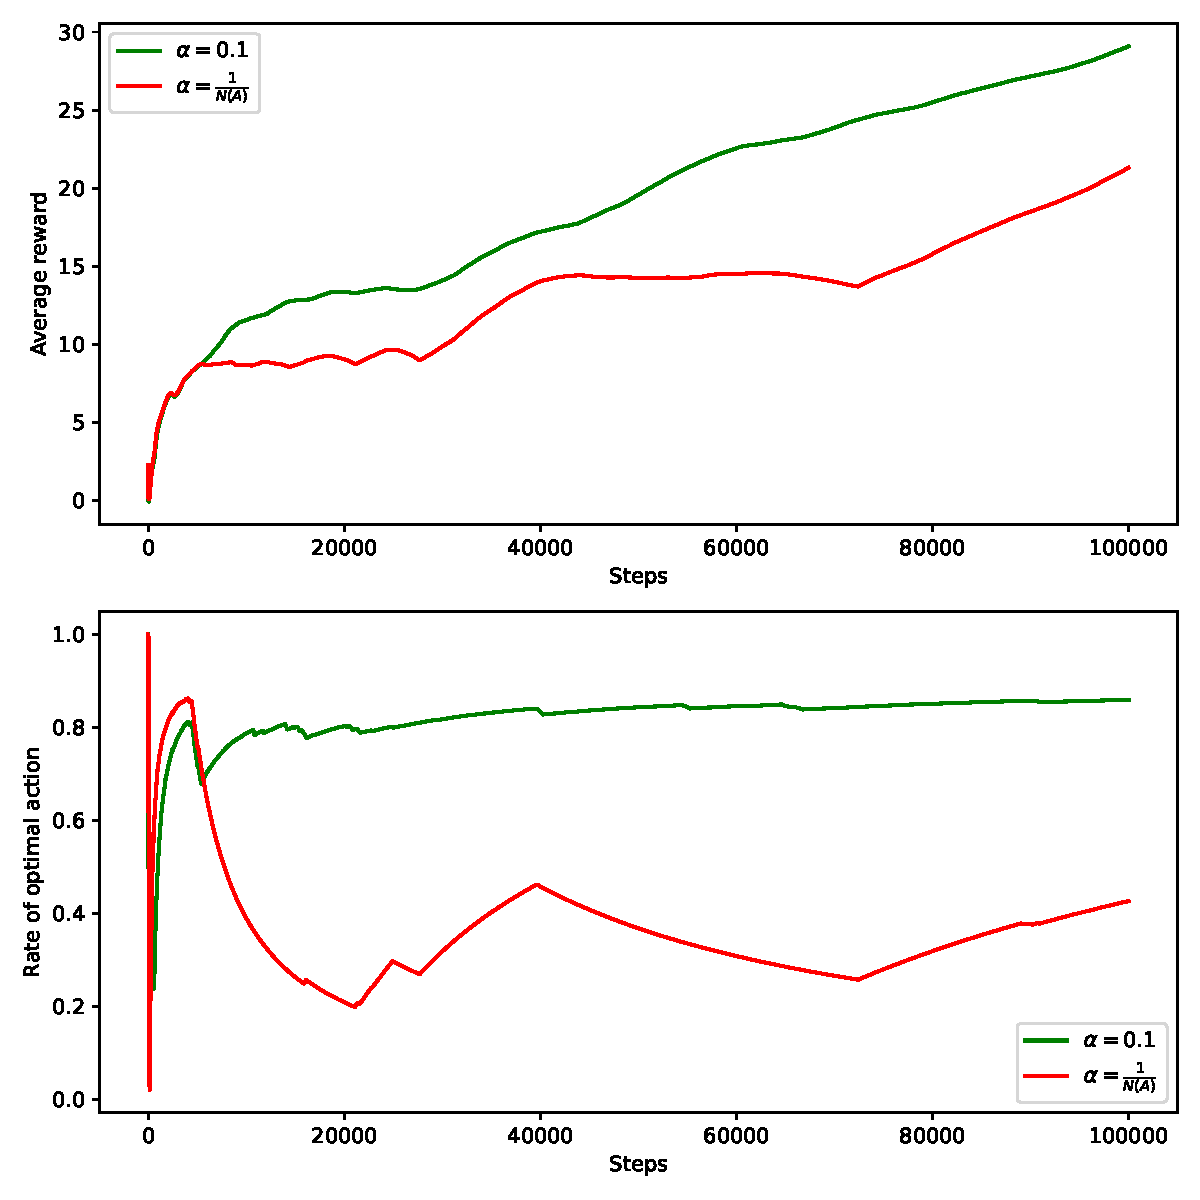
\includegraphics[width=\textwidth, angle=0]{chapters_latex/figures/ex_02_05.pdf}


\subsection*{Exercise 2.6: Mysterious Spikes} 
The results shown in Figure 2.3 should be quite reliable
because they are averages over 2000 individual, randomly chosen 10-armed bandit tasks.
Why, then, are there oscillations and spikes in the early part of the curve for the optimistic
method? In other words, what might make this method perform particularly better or
worse, on average, on particular early steps?

\subsubsection*{Solution:}

The agent might choose the optimal action correctly, then through chance it could receive high rewards initially, so it will choose it many times, thus increasing the \% Optimal rate. After a while, again by chance, its estimate of the reward could decrease, so it would choose another suboptimal action, and the \% Optimal action would decrease. 


\subsection*{Exercise 2.7: Unbiased Constant-Step-Size Trick} 
In most of this chapter we have used
sample averages to estimate action values because sample averages do not produce the
initial bias that constant step sizes do (see the analysis leading to (2.6)). However, sample
averages are not a completely satisfactory solution because they may perform poorly
on nonstationary problems. Is it possible to avoid the bias of constant step sizes while
retaining their advantages on nonstationary problems? One way is to use a step size of
\begin{equation}
    \beta_t \doteq \alpha / \bar{o}_t,
\end{equation}
where $\alpha > 0$ is a conventional constant step size and $\bar{o}_t$ is a trace of one that starts at 0:
\begin{equation}
    \bar{o}_{t+1} = \bar{o}_t + \alpha (1 - \bar{o}_t)
\end{equation}
for $t \geq 1$ and with $\bar{o}_1 \doteq \alpha$. 

Carry out an analysis like that in (2.6) to show that $Q_n$ is an exponential recency-weighted average without initial bias.

\subsubsection*{Solution:}


$\bar{o}_{t+1} = \bar{o}_t + \alpha (1 - \bar{o}_t) = \bar{o}_t(1-\alpha) + \alpha $

\begin{equation}
    \begin{aligned}
        \bar{o}_{1} &= \alpha \\
        \bar{o}_{2} &= \alpha + \alpha(1- \alpha) = 2\alpha - \alpha^2 \\
        \bar{o}_{t} &= \sum_{i=1}^{t} \alpha (1-\alpha)^{t-i}\\
        &=1-\left(1-\alpha\right)^{t}\\
    \end{aligned}
\end{equation}

\begin{equation}
    \begin{aligned}
        Q_{n+1} &= Q_n + \beta_n \left[ R_n - Q_n \right] \\
        &= Q_n + \frac{\alpha}{1-\left(1-\alpha\right)^{n}} \left[ R_n - Q_n \right] \\
        %&= \left( \prod_{i=1}^{n} (1-\beta_i) \right) Q_1 + \sum_{i=1}^{n} \beta_i R_i \prod_{k=i+1}^{n} (1-\beta_k) \\ 
        %&= \left( \prod_{i=1}^{n} (1-\alpha / \bar{o}_i) \right) Q_1 + \sum_{i=1}^{n} \alpha / \bar{o}_i R_i \prod_{k=i+1}^{n} (1-\alpha / \bar{o}_k) \\
    \end{aligned}
\end{equation}

The $\beta_n$ is decreasing, so it is recency-weighted. The contribution of the initial estimate $Q_1$ diminishes to zero as $t$ increases, the system effectively forgets the initial bias after a sufficient number of updates.

\subsection*{Exercise 2.8: UCB Spikes}
In Figure 2.4 the UCB algorithm shows a distinct spike
in performance on the 11th step. Why is this? Note that for your answer to be fully
satisfactory it must explain both why the reward increases on the 11th step and why it
decreases on the subsequent steps. Hint: If $c = 1$, then the spike is less prominent.

\subsubsection*{Solution:}


At the timesteps $t \leq 10$ there is always an action $a$ for which $N_t(a) = 0$, so the agent will always choose that action. After the 10th step the agent will choose greedily so the average reward increases. After some timesteps the uncertainty term of some other action overtakes the previously chosen action, and the agent starts to explore again, so the average reward decreases.

\subsection*{Exercise 2.9}
Show that in the case of two actions, the soft-max distribution is the same
as that given by the logistic, or sigmoid, function often used in statistics and artificial
neural networks.

\subsubsection*{Solution:}


\begin{equation}
    \begin{aligned}
        P(A_t = 1) &= \frac{e^{H_t(1)}}{\sum_{b=1}^{2} e^{H_t(b)}} = \frac{e^{H_t(1)}}{e^{H_t(1)} + e^{H_t(0)}} = \frac{1}{1 + e^{-(H_t(1)-H_t(0))}} \\
        &= \sigma(H_t(1)-H_t(0))
    \end{aligned}
\end{equation}


\subsection*{Exercise 2.10}
Suppose you face a 2-armed bandit task whose true action values change
randomly from time step to time step. Specifically, suppose that, for any time step,
the true values of actions 1 and 2 are respectively 10 and 20 with probability 0.5 (case
A), and 90 and 80 with probability 0.5 (case B). If you are not able to tell which case
you face at any step, what is the best expected reward you can achieve and how should
you behave to achieve it? Now suppose that on each step you are told whether you are
facing case A or case B (although you still don't know the true action values). This is an
associative search task. What is the best expected reward you can achieve in this task,
and how should you behave to achieve it?

\subsubsection*{Solution:}
If we can't differentiate the 2 cases:

Suppose the agent chooses action 1 with probability $p$. Then the expected reward is:
\begin{equation}
    \begin{aligned}
    \mathbb{E}[R] &= P(A) \cdot \left( p R_A(1) + (1-p)  R_A(2) \right) + 
                    P(B) \cdot \left( p R_B(1) + (1-p)  R_B(2) \right)\\
        &= 0.5 (10p + 20(1-p)) + 0.5 (90p + 80(1-p)) \\
        &= 50
    \end{aligned}
\end{equation}

If we \emph{can} differentiate the 2 cases:

We want to maximize the reward, so in case A the agent should choose action 2 and in case B it should choose action 1.   
\begin{equation}
    \begin{aligned}
    \mathbb{E}[R] &= P(A) \cdot R_A(2) + P(B) \cdot R_B(1) \\
        &= 0.5 \cdot 20 + 0.5 \cdot 90 \\
        &= 55
    \end{aligned}
\end{equation}


\subsection*{Exercise 2.11 (programming)}
Make a figure analogous to Figure 2.6 for the nonstationary
case outlined in Exercise 2.5. Include the constant-step-size $\varepsilon$-greedy algorithm with
$\alpha = 0.1$. Use runs of 200,000 steps and, as a performance measure for each algorithm and
parameter setting, use the average reward over the last 100,000 steps.

\subsubsection*{Solution:}

See the notebook. \\
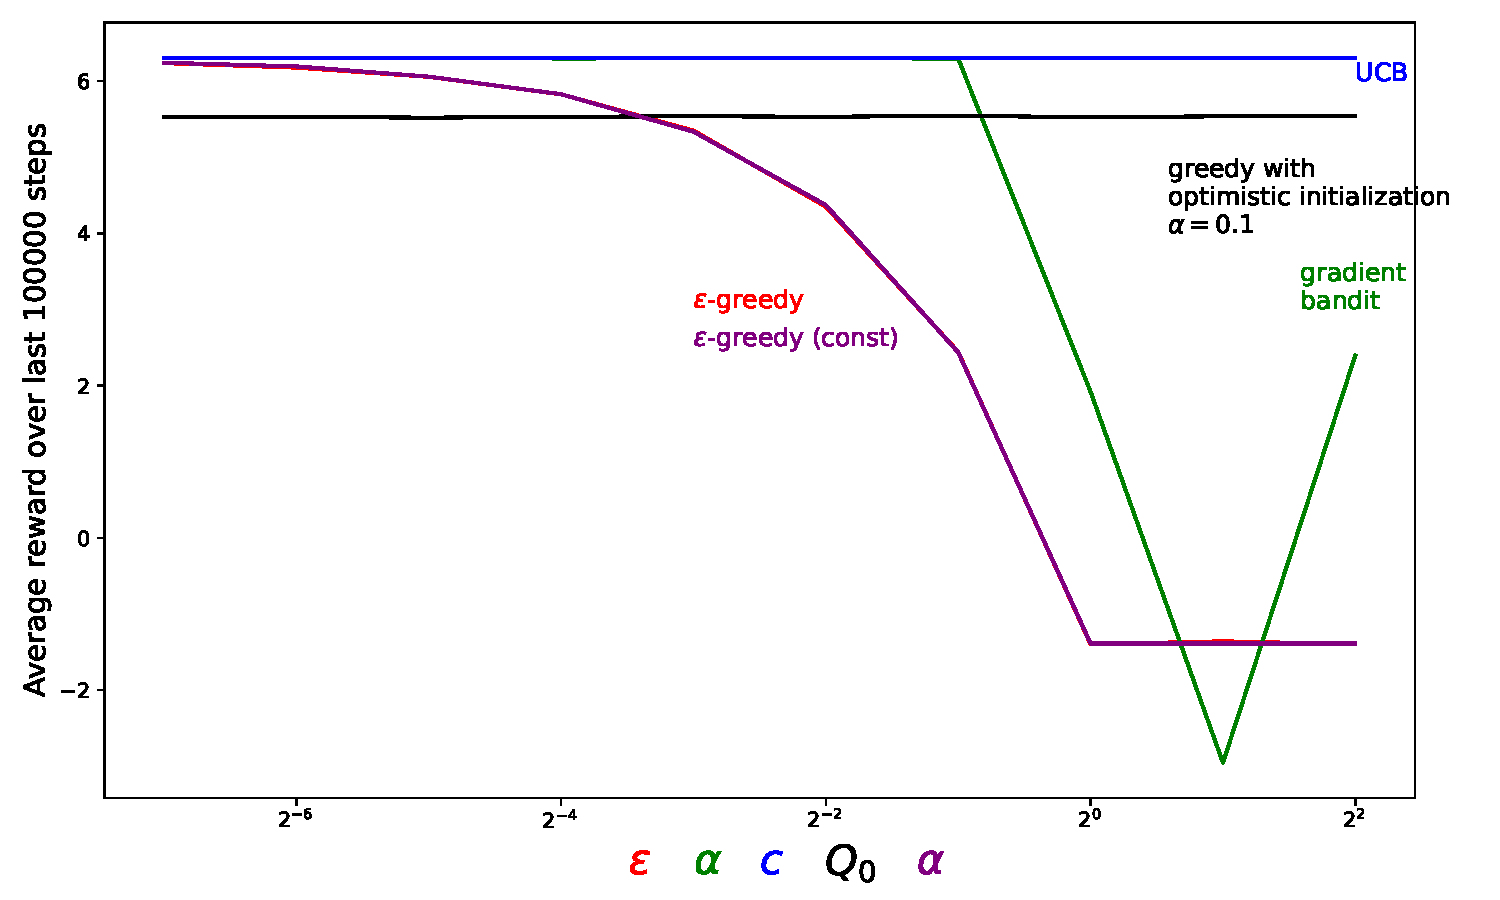
\includegraphics[width=\textwidth, angle=0]{chapters_latex/figures/ex_02_11_reward.pdf}
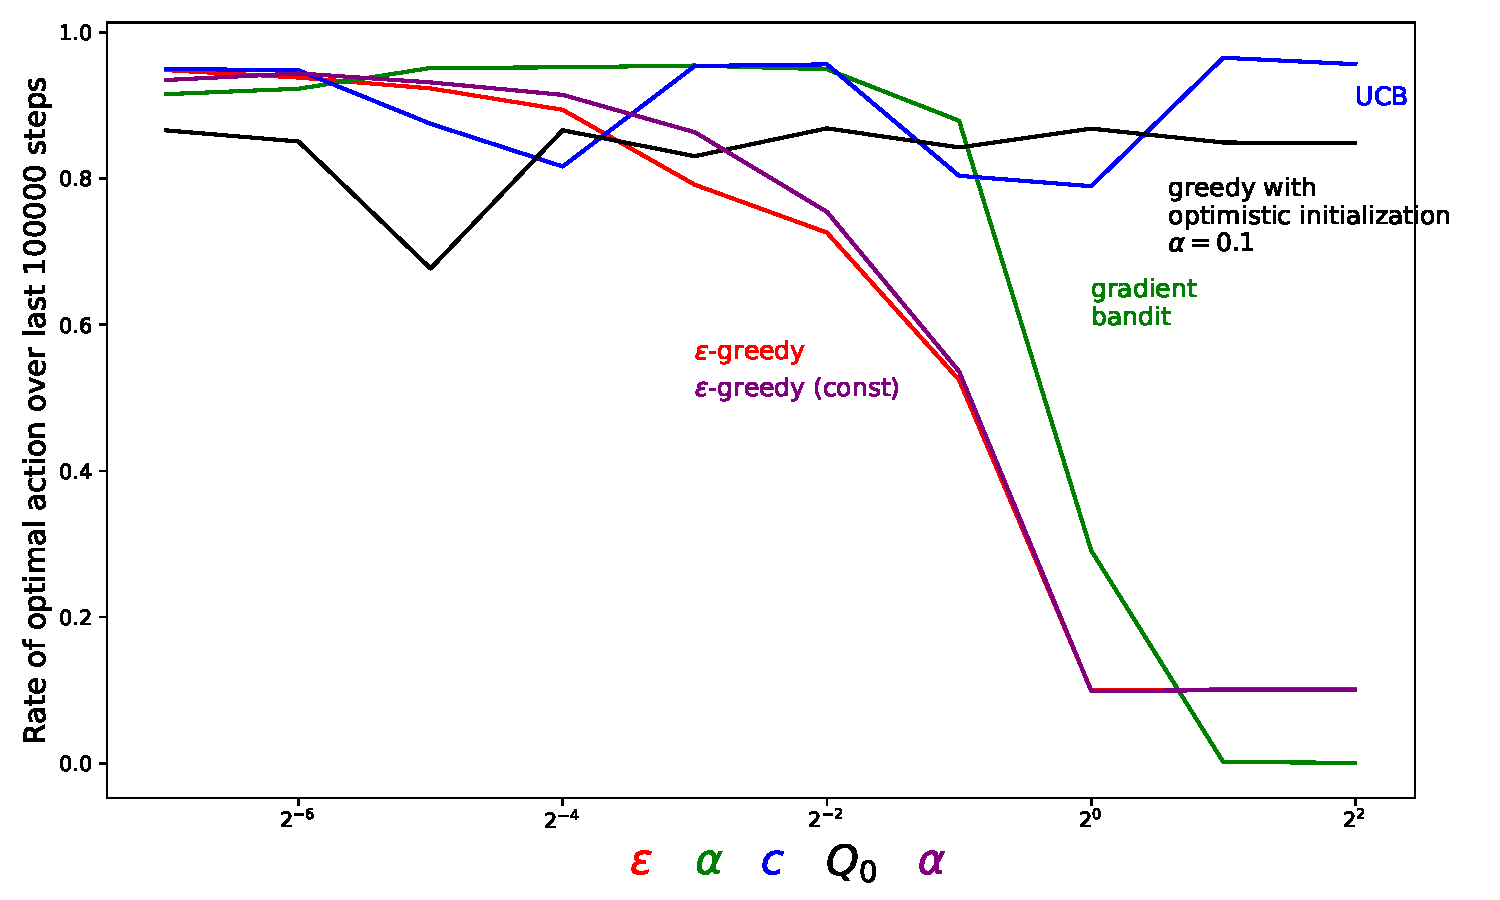
\includegraphics[width=\textwidth, angle=0]{chapters_latex/figures/ex_02_11_rate.pdf}

\section*{Chapter 3}

\subsection*{Exercise 3.1}
Devise three example tasks of your own that fit into the MDP framework,
identifying for each its states, actions, and rewards. Make the three examples as different
from each other as possible. The framework is abstract and flexible and can be applied in
many different ways. Stretch its limits in some way in at least one of your examples.

\subsubsection*{Solution:}
Example 1: Chess Player Program\\
Task Description: A chess-playing program aims to play chess in a way that conceals its identity as a non-human player.

\begin{itemize}
    \item \textbf{States (S):}
    \begin{itemize}
        \item Current board position (the arrangement of pieces).
        \item Time remaining for each player.
        \item Opponent's previous move history.
    \end{itemize}
    
    \item \textbf{Actions (A):}
    \begin{itemize}
        \item Make a legal move
        \item Pause (to simulate human behavior, potentially to analyze).
        \item Offer a draw or resignation.
    \end{itemize}
    
    \item \textbf{Rewards (R):}
    \begin{itemize}
        \item +1 for winning the game.
        \item -1 for drawing or losing.
        \item -0.01 for making moves that are too optimal, which might reveal the program's identity (e.g., moving in a way that a human wouldn't).
        \item +0.01 for making "human-like" moves (less optimal but more deceptive).
    \end{itemize}
\end{itemize}

Example 2: Person Taking an IQ Test\\
Task Description: A person takes an IQ test with the goal of maximizing their score.

\begin{itemize}
    \item \textbf{States (S):}
    \begin{itemize}
        \item Current question number.
        \item The question itself.
        \item Time left for the test.
    \end{itemize}
    
    \item \textbf{Actions (A):}
    \begin{itemize}
        \item Answer the question (select one of multiple-choice options).
        \item Think.
        \item Skip the question.
    \end{itemize}
    
    \item \textbf{Rewards (R):}
    \begin{itemize}
        \item +1 for a correct answer.
        \item 0 for a skipped question.
        \item -1 for an incorrect answer.
    \end{itemize}
\end{itemize}

Example 3: Elevator Control System\\
Task Description: An elevator system optimizes its operation to minimize wait times and maximize efficiency in a multi-story building.

\begin{itemize}
    \item \textbf{States (S):}
    \begin{itemize}
        \item Current floor of the elevator.
        \item Status of the elevator (moving up, moving down, idle).
        \item Status of the door (open, closed)
        \item Floors where people wish to go up.
        \item Floors where people wish to go down.
        \item Current load (number of passengers in the elevator based on weight).
        \item Buttons pressed (which floors the passengers in the elevator wish to go to).
    \end{itemize}
    
    \item \textbf{Actions (A):}
    \begin{itemize}
        \item Move up.
        \item Move down.
        \item Open doors.
        \item Close doors.
        \item Wait on the current floor.
    \end{itemize}
    
    \item \textbf{Rewards (R):}
    \begin{itemize}
        \item -1 for each second the passengers spend waiting.
        \item -1 for unnecessary movements (e.g., moving to a floor with no waiting passengers).
    \end{itemize}
\end{itemize}


\subsection*{Exercise 3.2}
Is the MDP framework adequate to usefully represent all goal-directed learning tasks? Can you think of any clear exceptions?

\subsubsection*{Solution:}
There are situations where the MDP framework is not adequate. 
\begin{itemize}
    \item Continous action spaces
    \item Non-Markovian environments
    \item High-Dimensional state spaces
\end{itemize}

Example: self-driving for cars have continous action spaces (steering the wheel, rate of acceleration) and high-dimensional state spaces (images of the environment).

\subsection*{Exercise 3.3}
Consider the problem of driving. You could define the actions in terms of
the accelerator, steering wheel, and brake, that is, where your body meets the machine.
Or you could define them farther out—say, where the rubber meets the road, considering
your actions to be tire torques. Or you could define them farther in—say, where your
brain meets your body, the actions being muscle twitches to control your limbs. Or you
could go to a really high level and say that your actions are your choices of where to drive.
What is the right level, the right place to draw the line between agent and environment?
On what basis is one location of the line to be preferred over another? Is there any
fundamental reason for preferring one location over another, or is it a free choice?

\subsubsection*{Solution:} 
The right place to draw the line between agent and environment is highly dependant on the problem we are modeling/trying to solve. If we want to create a route finding algorithm, then the highest level of choice would be ideal, but if we want to look at the problem in a neuroscientific way, then the brain and muscle option would be fine.\\
There is no fundamental reason for preferring one location over another, it is only good for using the advantages of abstraction.


\subsection*{Exercise 3.4}
Give a table analogous to that in Example 3.3, but for $p(s', r |s, a)$ . It
should have columns for $s$, $a$, $s'$, $r$, and $p(s', r |s, a)$ , and a row for every 4-tuple for which
$p(s', r |s, a)  > 0$.

\subsubsection*{Solution:}

\begin{table}[h!]
    \centering
    \begin{tabular}{ll|ll|c}
        $s$  & $a$      & $s'$ & $r$                 & $p(s', r |s, a)$ \\ \hline
        high & search   & high & $r_{\text{search}}$ & $\alpha$         \\
        high & search   & low  & $r_{\text{search}}$ & $1 - \alpha$     \\
        low  & search   & high & -3                  & $1 - \beta$      \\
        low  & search   & low  & $r_{\text{search}}$ & $\beta$          \\
        high & wait     & high & $r_{\text{wait}}$   & 1                \\
        low  & wait     & low  & $r_{\text{wait}}$   & 1                \\
        low  & recharge & high & 0                   & 1               
    \end{tabular}
\end{table}


\subsection*{Exercise 3.5}
The equations in Section 3.1 are for the continuing case and need to be
modified (very slightly) to apply to episodic tasks. Show that you know the modifications
needed by giving the modified version of (3.3).

\subsubsection*{Solution:}
The original equation:
\[
\sum_{s' \in S} \sum_{r \in R} P(s', r \mid s, a) = 1, \quad \forall s \in S, \forall a \in A(s)
\]

This would exclude the terminal states $S^+ \setminus S$, so we wouldn't count the cases where a state goes from non-terminal to a terminal state.

The modified equation:
\[
\sum_{s' \in S^+} \sum_{r \in R} P(s', r \mid s, a) = 1, \quad \forall s \in S^+, \forall a \in A(s)
\]


\subsection*{Exercise 3.6}
Suppose you treated pole-balancing as an episodic task but also used
discounting, with all rewards zero except for  1 upon failure. What then would the
return be at each time? How does this return differ from that in the discounted, continuing
formulation of this task?

\subsubsection*{Solution:}

\[
G_t = \sum_{k=0}^{T-t} \gamma^k r_{t+k+1} = 0 + 0 + 0 + \dots + -\gamma^{T-t} = -\gamma^{T-t}
\]

The reward in the discounted, continuing formulation:

\[
G_t = \sum_{k \in K} -\gamma^{k-t}
\]

Where $K$ is the number of time steps before failure (as well as to the times of later failures).


\subsection*{Exercise 3.7} Imagine that you are designing a robot to run a maze. You decide to give it a
reward of +1 for escaping from the maze and a reward of zero at all other times. The task
seems to break down naturally into episodes—the successive runs through the maze—so
you decide to treat it as an episodic task, where the goal is to maximize expected total
reward (3.7). After running the learning agent for a while, you find that it is showing
no improvement in escaping from the maze. What is going wrong? Have you effectively
communicated to the agent what you want it to achieve?

\subsubsection*{Solution:}

The agent receives +1 reward regardless of the timesteps it takes it to leave the maze. Because of this, it can't distinguish a good policy from a bad one.

\subsection*{Exercise 3.8}
Suppose $\gamma = 0.5$ and the following sequence of rewards is received $R_1 = -1$, $R_2 = 2$, $R_3 = 6$, $R_4 = 3$, and $R_5 = 2$, with $T = 5$. What are $G_0$, $G_1$, $\dots$, $G_5$? Hint:
Work backwards.

\subsubsection*{Solution:}

\begin{equation}
    \begin{aligned}
        G_t &= R_{t+1} + \gamma G_{t+1} \\
        G_5 &= 0 \\
        G_4 &= 2 + 0.5 \cdot 0 = 2 \\
        G_3 &= 3 + 0.5 \cdot 2 = 4 \\
        G_2 &= 6 + 0.5 \cdot 4 = 8 \\
        G_1 &= 2 + 0.5 \cdot 8 = 6 \\
        G_0 &= -1 + 0.5 \cdot 6 = 2 
    \end{aligned}
\end{equation}


\subsection*{Exercise 3.9}
Suppose  $\gamma = 0.9$ and the reward sequence is $R_1 = 2$ followed by an infinite
sequence of 7s. What are $G_1$ and $G_0$? 

\subsubsection*{Solution:}

\[
G_0 = 2 + \sum_{k = 1}^{\infty} 0.9^k \cdot 7  = 2 + \frac{0.9 \cdot 7}{1-0.9} = 65
\]

\[
G_1 = \sum_{k = 0}^{\infty} 0.9^k \cdot 7 = \frac{7}{1-0.9} = 70
\]

\subsection*{Exercise 3.10}
Prove the second equality in (3.10).

\subsubsection*{Solution:}

The equality in question:

\[
\sum_{k = 0}^{\infty} \gamma^k = \frac{1}{1-\gamma}
\]

Proof:

\begin{align*}
    \sum_{k = 0}^{\infty} \gamma^k &= 1 + \gamma + \gamma^2 + \gamma^3 + \dots \\
    &= 1 + \gamma (1 + \gamma + \gamma^2  + \dots) \\
    &= 1 + \gamma \sum_{k = 0}^{\infty} \gamma^k
\end{align*}

\[
(1 - \gamma)\sum_{k = 0}^{\infty} \gamma^k = 1
\]

\[
\sum_{k = 0}^{\infty} \gamma^k = \frac{1}{1 - \gamma}
\]

\subsection*{Exercise 3.10}
If the current state is $S_t$, and actions are selected according to a stochastic
policy $\pi$, then what is the expectation of $R_{t+1}$ in terms of $\pi$ and the four-argument
function $p$ (3.2)?

\subsubsection*{Solution:}

\[
    \mathbb{E}_{\pi} \left[R_{t+1} | S_t = s \right] = \sum_r r  \sum_{s', a} \pi(a|s) p(s', r | s, a)
\]

\subsection*{Exercise 3.12}
Give an equation for $v_\pi$ in terms of $q_\pi$ and $\pi$.

\subsubsection*{Solution:}
\begin{align*}
    v_\pi(s)&=\mathbb{E}_{\pi} \left[G_{t+1} | S_t = s \right] \\
    &= \sum_a \mathbb{E}_{\pi} \left[G_{t+1} | S_t = s, A_t = a \right] \pi(a|s)\\
    &= \sum_a q_\pi(s,a) \pi(a|s)
\end{align*}

\subsection*{Exercise 3.13}
Give an equation for $q_\pi$ in terms of $v_\pi$ and the four-argument $p$.

\subsubsection*{Solution:}

\begin{align*}
    q_\pi(s, a) &= \mathbb{E}_{\pi} \left[G_{t+1} | S_t = s, A_t = a \right] \\
    &= \sum_{s',r} p(s', r | s, a) (r + \gamma \mathbb{E}_{\pi} \left[G_{t+2} | S_{t+1} = s' \right]) \\
    &= \sum_{s',r} p(s', r | s, a) (r + \gamma v_\pi(s'))
\end{align*}


\subsection*{Exercise 3.14}
The Bellman equation (3.14) must hold for each state for the value function
$v_\pi$ shown in Figure 3.2 (right) of Example 3.5. Show numerically that this equation holds
for the center state, valued at $+0.7$, with respect to its four neighboring states, valued at
$+2.3$, $+0.4$,  $-0.4$, and $+0.7$. (These numbers are accurate only to one decimal place.)

\subsubsection*{Solution:}

\begin{align*}
    v_\pi(s) &= \sum_a \pi(a|s) \sum_{s',r} p(s',r |s, a)\left[r + \gamma v_\pi(s')\right] \\
    &= 0.25 \cdot 0.9 \cdot (2.3 + 0.4 - 0.4 + 0.7) \\
    &= 0.675
\end{align*}

\subsection*{Exercise 3.15}
In the gridworld example, rewards are positive for goals, negative for
running into the edge of the world, and zero the rest of the time. Are the signs of these
rewards important, or only the intervals between them? Prove, using (3.8), that adding a
constant $c$ to all the rewards adds a constant, $v_c$, to the values of all states, and thus
does not affect the relative values of any states under any policies. What is $v_c$ in terms
of $c$ and $\gamma$? 

\subsubsection*{Solution:}
\begin{align*}
    G_t' &= \sum_{k=0}^{\infty}\gamma^k (R_{t+k+1}+c) \\
    &= \sum_{k=0}^{\infty}\gamma^k R_{t+k+1} + c \sum_{k=0}^{\infty}\gamma^k \\
    &= G_t + \frac{c}{1 - \gamma}
\end{align*}

\subsection*{Exercise 3.16}
Now consider adding a constant $c$ to all the rewards in an episodic task,
such as maze running. Would this have any effect, or would it leave the task unchanged
as in the continuing task above? Why or why not? Give an example.

\subsubsection*{Solution:}
This could have an adverse effect for the task. The maze running example could be formulated as the agent getting a -1 reward every timestep while still in the maze, and a 0 reward when reaching the exit. Adding a $c > 1$ constant to every reward would mean that the agent is incentivised to stay in the maze and avoid the exit.

\subsection*{Exercise 3.17}
What is the Bellman equation for action values, that
is, for $q_\pi$? It must give the action value $q_\pi(s,a)$ in terms of the action
values, $q_\pi(s',a')$, of possible successors to the state-action pair $(s,a)$.
Hint: The backup diagram to the right corresponds to this equation.
Show the sequence of equations analogous to (3.14), but for action
values.

\subsubsection*{Solution:}

\begin{align*}
    q_\pi(s, a) &= \mathbb{E}_{\pi} \left[G_{t+1} | S_t = s, A_t = a \right] \\
    &= \sum_{s',r} p(s', r | s, a) \left(r + \gamma \sum_{a'} \pi(a'|s') \mathbb{E}_{\pi} \left[G_{t+2} | S_{t+1} = s', A_{t+1} = a' \right]\right) \\
    &= \sum_{s',r} p(s', r | s, a) \left(r + \gamma \sum_{a'} \pi(a'|s') q_\pi(s',a')\right)
\end{align*}

\subsection*{Exercise 3.18}
The value of a state depends on the values of the actions possible in that
state and on how likely each action is to be taken under the current policy. We can
think of this in terms of a small backup diagram rooted at the state and considering each
possible action:

\begin{center}
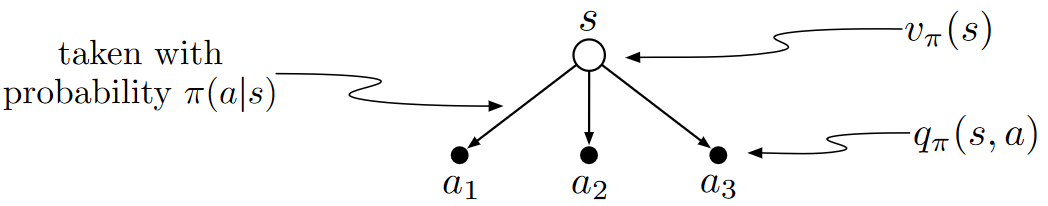
\includegraphics[width=0.8\textwidth]{chapters_latex/figures/ex_03_18.png}
\end{center}

Give the equation corresponding to this intuition and diagram for the value at the root
node, $v_\pi(s)$, in terms of the value at the expected leaf node, $q_\pi(s,a)$, given $S_t = s$. This
equation should include an expectation conditioned on following the policy, $\pi$. Then give
a second equation in which the expected value is written out explicitly in terms of $\pi(a|s)$
such that no expected value notation appears in the equation.

\subsubsection*{Solution:}

\[
    v_\pi(s)= \mathbb{E}_{\pi} \left[q_\pi(s,a) | S_t = s \right]
\]

\[
    v_\pi(s)= \sum_a \pi(a|s) q_\pi(s,a)
\]

\subsection*{Exercise 3.19} The value of an action, $q_\pi(s,a)$, depends on the expected next reward and
the expected sum of the remaining rewards. Again we can think of this in terms of a
small backup diagram, this one rooted at an action (state-action pair) and branching to
the possible next states:

\begin{center}
    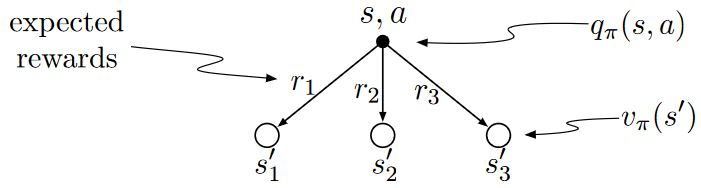
\includegraphics[width=0.6\textwidth]{chapters_latex/figures/ex_03_19.png}
\end{center}

Give the equation corresponding to this intuition and diagram for the action value,
$q_\pi(s,a)$, in terms of the expected next reward, $R_{t+1}$, and the expected next state value,
$v_\pi(S_{t+1})$, given that $S_t = s$ and $A_t = a$. This equation should include an expectation but
not one conditioned on following the policy. Then give a second equation, writing out the
expected value explicitly in terms of $p(s',r|s,a)$ defined by (3.2), such that no expected
value notation appears in the equation. 

\subsubsection*{Solution:}

\[
    q_\pi(s, a)= \mathbb{E} \left[R_{t+1} + \gamma v_\pi(S_{t+1}) | S_t = s, A_t = a \right]
\]

\[
    q_\pi(s, a)= \sum_{s',r} p(s',r|s,a) \left( r + \gamma v_\pi(s') \right)
\]


\subsection*{Exercise 3.20}
Draw or describe the optimal state-value function for the golf example.

\subsubsection*{Solution:}
Use the putter when on the green, use the driver in the other cases.
\begin{center}
    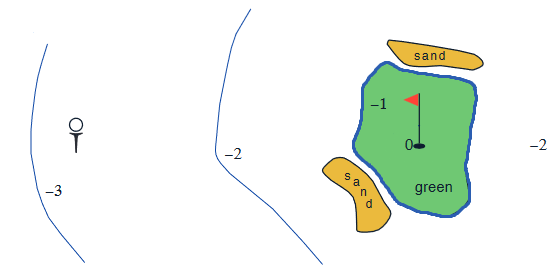
\includegraphics[width=0.6\textwidth]{chapters_latex/figures/ex_03_20.png}
\end{center}

\subsection*{Exercise 3.21} 
Draw or describe the contours of the optimal action-value function for putting,
$q_*(s, \text{putter})$, for the golf example.

\subsubsection*{Solution:}
$q_*(s, \text{putter})$ is equal to $1 + v_*(s')$ where $s'$ is the new location of the ball. If the ball arrives at the green, the next action should be using a putter, else the agent should use a driver.
\begin{center}
    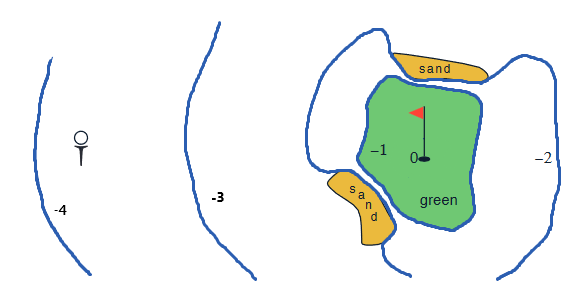
\includegraphics[width=0.6\textwidth]{chapters_latex/figures/ex_03_21.png}
\end{center}

\subsection*{Exercise 3.22}
Consider the continuing MDP shown to the
right. The only decision to be made is that in the top state,
where two actions are available, left and right. The numbers
show the rewards that are received deterministically after
each action. There are exactly two deterministic policies,
$\pi_\text{left}$ and $\pi_\text{right}$. What policy is optimal if  $\gamma = 0$? If  $\gamma = 0.9$?
If  $\gamma = 0.5$?
\begin{center}
    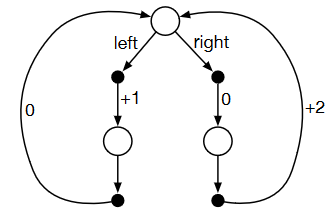
\includegraphics[width=0.6\textwidth]{chapters_latex/figures/ex_03_22.png}
\end{center}

\subsubsection*{Solution:}

After 2 actions the state will return to the original state, so $R_n = R_{n+2}$

\[
G_t = R_{t+1} + \gamma R_{t+2} + \gamma^2 G_t
\]

\[
(1 - \gamma^2) G = R_{t+1} + \gamma R_{t+2}
\]

\[
G_t = \frac{R_{t+1} + \gamma R_{t+2}}{1 - \gamma^2}
\]

$\pi_{\text{right}}$:   $G_t = \frac{2 \gamma}{1 - \gamma^2} $

$\pi_{\text{left}}$:   $G_t = \frac{1}{1 - \gamma^2} $

The optimal policy maximizes the value function, and because there is no stochasticity, $G_t = v_{\pi}(s)$.

If $(2\gamma > 1)$, going right is the optimal policy, while in the case of $(2\gamma < 1)$, going left is optimal.

For $(\gamma = 0)$: left is the optimal policy.

For $(\gamma = 0.9)$: right is the optimal policy.

For $(\gamma = 0.5)$: both policies are optimal.

\subsection*{Exercise 3.23}
Give the Bellman equation for $q_*$ for the recycling robot.

\subsubsection*{Solution:}

\begin{align*}
    q_*(\text{high}, \text{search}) &= r_\text{search} + \gamma \left( \alpha \max_a q_*(\text{high}, a) + (1 - \alpha) \max_a q_*(\text{low}, a) \right) \\
    q_*(\text{high}, \text{wait}) &= r_\text{wait} + \gamma \max_aq_*(\text{high}, a) \\
    q_*(\text{low}, \text{search}) &= \beta \left( r_\text{search} + \gamma  \max_a q_*(\text{low}, a) \right) \\
    &\quad + (1 - \beta) \left(-3 + \max_a q_*(\text{high}, a) \right) \\
    q_*(\text{low}, \text{wait}) &= r_\text{wait} + \gamma \max_aq_*(\text{low}, a) \\
    q_*(\text{low}, \text{recharge}) &= \gamma \max_aq_*(\text{high}, a)
\end{align*}

\subsection*{Exercise 3.24}
Figure 3.5 gives the optimal value of the best state of the gridworld as
24.4, to one decimal place. Use your knowledge of the optimal policy and (3.8) to express
this value symbolically, and then to compute it to three decimal places. 

\subsubsection*{Solution:}

\[
G_t = 10 + 0 + 0 + 0 + 0 + 0.9^5 \cdot G_t
\]
\[
G_t = \frac{10}{1-0.9^5} = 24.419
\]


\subsection*{Exercise 3.25}
Give an equation for $v_*$ in terms of $q_*$.

\subsubsection*{Solution:}

\[
v_*(s) = \max_a q_*(s,a)
\]

\subsection*{Exercise 3.26}
Give an equation for $q_*$ in terms of $v_*$ and the four-argument $p$.

\subsubsection*{Solution:}

\[
q_*(s,a) = \sum_{s', r} p(s', r |s, a)  \left( r + \gamma v_*(s') \right)
\]

\subsection*{Exercise 3.27}
Give an equation for $\pi_*$ in terms of $q_*$.

\subsubsection*{Solution:}

\[
\pi_*(a|s) =
    \begin{cases}
        1,  & \text{if } a = \argmax_a q_*(s,a)\\
        0,  & \text{else}
    \end{cases}
\]


\subsection*{Exercise 3.28}
Give an equation for $\pi_*$ in terms of $v_*$ and the four-argument $p$.

\subsubsection*{Solution:}

\[
\pi_*(a|s) =
    \begin{cases}
        1,  & \text{if } a = \argmax_a \sum_{s', r} p(s', r |s, a)  \left( r + \gamma v_*(s') \right)\\
        0,  & \text{else}
    \end{cases}
\]

\subsection*{Exercise 3.29}
Rewrite the four Bellman equations for the four value functions ($v_\pi$, $v_*$, $q_\pi$, $q_*$)
in terms of the three argument function $p$ (3.4) and the two-argument function $r$ (3.5).

\subsubsection*{Solution:}

\[
q_\pi(s,a) = r(s,a) + \gamma \sum_{s',a'} p(s'|s,a) \pi(a'|s') q _\pi(s',a')
\]

\[
    q_*(s,a) = r(s,a) + \gamma  \sum_{s'} p(s'|s,a) \max_{a'} \pi(a'|s') q _*(s',a')
\]

\[
    v_\pi(s) = \sum_a \pi(a|s) \left( r(s,a) + \gamma \sum_{s'} p(s'|s,a) v_\pi(s') \right) 
\]

\[
    v_*(s) = \max_a  r(s,a) + \gamma \sum_{s'} p(s'|s,a) v_*(s') 
\]
\section*{Chapter 4}

\subsection*{Exercise 4.1}

\subsubsection*{Solution:}
In Example 4.1, if $\pi$ is the equiprobable random policy, what is $q_\pi(11, \text{down})$?
What is $q_\pi(7, \text{down})$?

\[
q_\pi(11, \text{down}) = r + v_\pi(\text{end state}) = -1 + 0 = -1
\]

\[
q_\pi(7, \text{down}) = r + v_\pi(11) = -1 - 14 = -15
\]


\subsection*{Exercise 4.2}
In Example 4.1, suppose a new state 15 is added to the gridworld just below
state 13, and its actions, left, up, right, and down, take the agent to states 12, 13, 14,
and 15, respectively. Assume that the transitions from the original states are unchanged.
What, then, is $v_\pi(15)$ for the equiprobable random policy? Now suppose the dynamics of
state 13 are also changed, such that action down from state 13 takes the agent to the new
state 15. What is $v_\pi(15)$ for the equiprobable random policy in this case?

\subsubsection*{Solution:}
First case:
\[
v_\pi(15) = -1 + 0.25(v_\pi(12) + v_\pi(13) + v_\pi(14) + v_\pi(15))
\]

\[
v_\pi(15) = -\frac{4}{3} + \frac{1}{3}(v_\pi(12) + v_\pi(13) + v_\pi(14) ) = -\frac{4}{3} + \frac{1}{3}(-22 - 20 - 14) = -20
\]

Second case:

Using the iterative method with $v_\pi^1(15) = -20$.
\begin{align*}
v_\pi^1(13) &= -1 + 0.25(v_\pi(12) + v_\pi(9) + v_\pi(14) + v_\pi(15)) \\
&= -1 + 0.25(-22 - 20 - 14 - 20) = -20
\end{align*}

The $v(s)$ values didn't change, so the iterative algorithm can terminate here, $v_\pi(15) = -20$.

\subsection*{Exercise 4.3}
What are the equations analogous to (4.3), (4.4), and (4.5), but for action-
value functions instead of state-value functions?

\subsubsection*{Solution:}

\begin{align*}
    q_\pi(s, a) &= \mathbb{E} \left[R_{t+1} + \gamma \sum_{a'} \pi(a' \mid S_{t+1}) q_\pi(S_{t+1}, a') \middle| S_t = s, A_t = a \right] \\
    &= \sum_{s',r} p(s', r \mid s, a) \left(r + \gamma \sum_{a'} \pi(a'\mid s') q_\pi(s', a') \right)
\end{align*}

\[
    q_{k+1}(s, a) = \sum_{s',r} p(s', r \mid s, a) \left(r + \gamma \sum_{a'} \pi(a' \mid s') q_{k}(s', a') \right) 
\]

\subsection*{Exercise 4.4}
The policy iteration algorithm on page 80 has a subtle bug in that it may
never terminate if the policy continually switches between two or more policies that are
equally good. This is okay for pedagogy, but not for actual use. Modify the pseudocode
so that convergence is guaranteed.

\subsubsection*{Solution:}

Instead of 
\[
    \pi(s) \leftarrow \argmax_a \sum_{s',r} p(s',r \mid s,a)[r + \gamma V(s')]
\]

Use:

\[
    \pi(s) \leftarrow \min\{ a \in \argmax_a \sum_{s',r} p(s',r \mid s,a)[r + \gamma V(s')] \}
\]

This way if there are multiple policies that are equally good, the agent always chooses the action with the lowest value. We could also check if $q_\pi(s,\pi(s)) == q_\pi(s,a)$.

\subsection*{Exercise 4.5}
How would policy iteration be defined for action values? Give a complete
algorithm for computing $q_*$, analogous to that on page 80 for computing $v_*$. Please pay
special attention to this exercise, because the ideas involved will be used throughout the
rest of the book.

\subsubsection*{Solution:}
\fbox{
\begin{minipage}{0.95\textwidth}
\footnotesize 
\begin{enumerate}
    \item \textbf{Initialization}\\
    $Q(s,a) \in \mathbb{R}$ and $\pi(s) \in A(s)$ arbitrarily for all $s \in S$; $Q(\text{terminal}, a) \doteq 0$

    \item \textbf{Policy Evaluation}\\
    Loop: 
    \begin{itemize}
        \item[] $\Delta \leftarrow 0$
        \item[] Loop for each $s \in S$:
        \begin{itemize}
            \item[] Loop for each $a \in A(s)$:
            \begin{itemize}
                \item[] $q \leftarrow Q(s,a)$
                \item[] $Q(s,a) \leftarrow \sum_{s',r} p(s', r \mid s, a) [r + \gamma Q(s', \pi(s'))]$
                \item[] $\Delta \leftarrow \max(\Delta, |q - Q(s,a)|)$
            \end{itemize}
        \end{itemize}
    \end{itemize}
    until $\Delta < \theta$ (a small positive number determining the accuracy of estimation)

    \item \textbf{Policy Improvement}
    \begin{itemize}
        \item[] $\textit{policy-stable} \leftarrow \textit{true}$
        \item[] For each $s \in S$:
        \begin{itemize}
            \item[] $\textit{old-action} \leftarrow \pi(s)$
            \item[] $\pi(s) \leftarrow \argmax_a Q(s,a) $
            \item[] If $\textit{old-action} \neq \pi(s)$, then $\textit{policy-stable} \leftarrow \textit{false}$
        \end{itemize}
    \end{itemize}
    If $\textit{policy-stable}$, then stop and return $Q \approx q_*$ and $\pi \approx \pi_*$; else go to 2
\end{enumerate}
\end{minipage}
}

\subsection*{Exercise 4.6}
Suppose you are restricted to considering only policies that are $\varepsilon$-soft,
meaning that the probability of selecting each action in each state, $s$, is at least $\varepsilon/|A(s)|$.
Describe qualitatively the changes that would be required in each of the steps 3, 2, and 1,
in that order, of the policy iteration algorithm for $v_*$ on page 80.

\subsubsection*{Solution:}

\begin{enumerate}
    \item $\pi(a \mid s) = 1/|A(s)|$
    \item $V(s) \leftarrow \sum_a \pi(a \mid s) \sum_{s',r} p(s',r \mid s, a) (r + \gamma V(s'))$
    \item \footnotesize $
    \pi(a \mid s) =
        \begin{cases}
            1-\varepsilon + \frac{\varepsilon}{|A(s)|},  & \text{if } a = \arg \max_a \sum_{s',r} p(s', r \mid s, a) [r + \gamma V(s')]\\
            \frac{\varepsilon}{|A(s)|},  & \text{else}
        \end{cases}
    $
\end{enumerate}

\subsection*{Exercise 4.7 (programming)}
Write a program for policy iteration and re-solve Jack's car
rental problem with the following changes. One of Jack's employees at the first location
rides a bus home each night and lives near the second location. She is happy to shuttle
one car to the second location for free. Each additional car still costs \$2, as do all cars
moved in the other direction. In addition, Jack has limited parking space at each location.
If more than 10 cars are kept overnight at a location (after any moving of cars), then an
additional cost of \$4 must be incurred to use a second parking lot (independent of how
many cars are kept there). These sorts of nonlinearities and arbitrary dynamics often
occur in real problems and cannot easily be handled by optimization methods other than
dynamic programming. To check your program, first replicate the results given for the
original problem.

\subsubsection*{Solution:}

See the notebooks.

\begin{figure}[H]
    \centering
    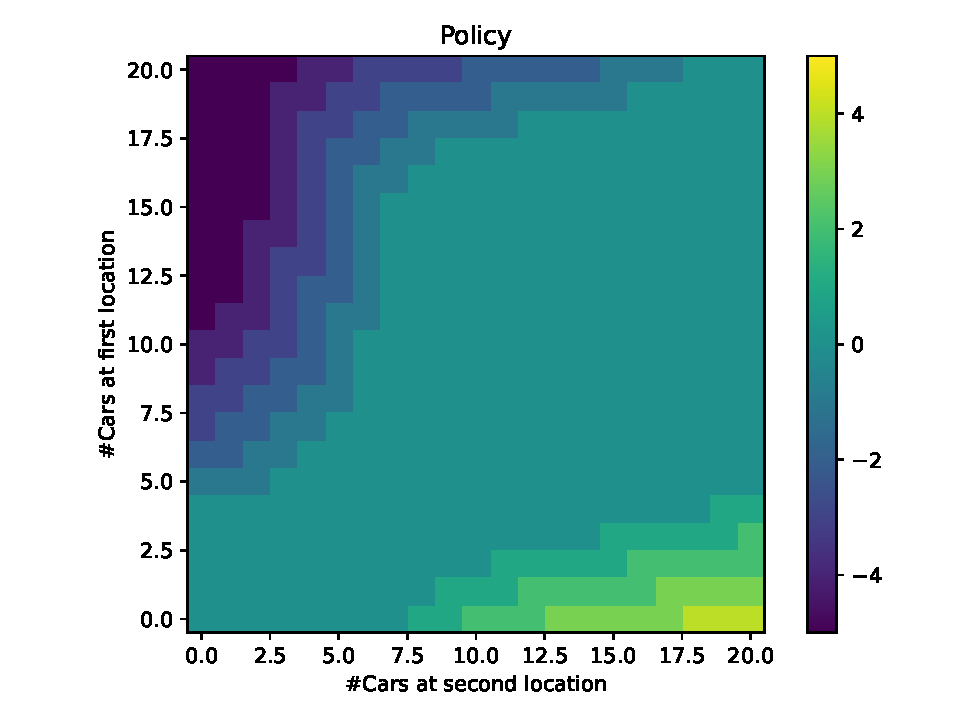
\includegraphics[width=0.8\textwidth]{chapters_latex/figures/ex_04_07_original.pdf}
    \caption{The original policy.}
\end{figure}

\begin{figure}[H]
    \centering
    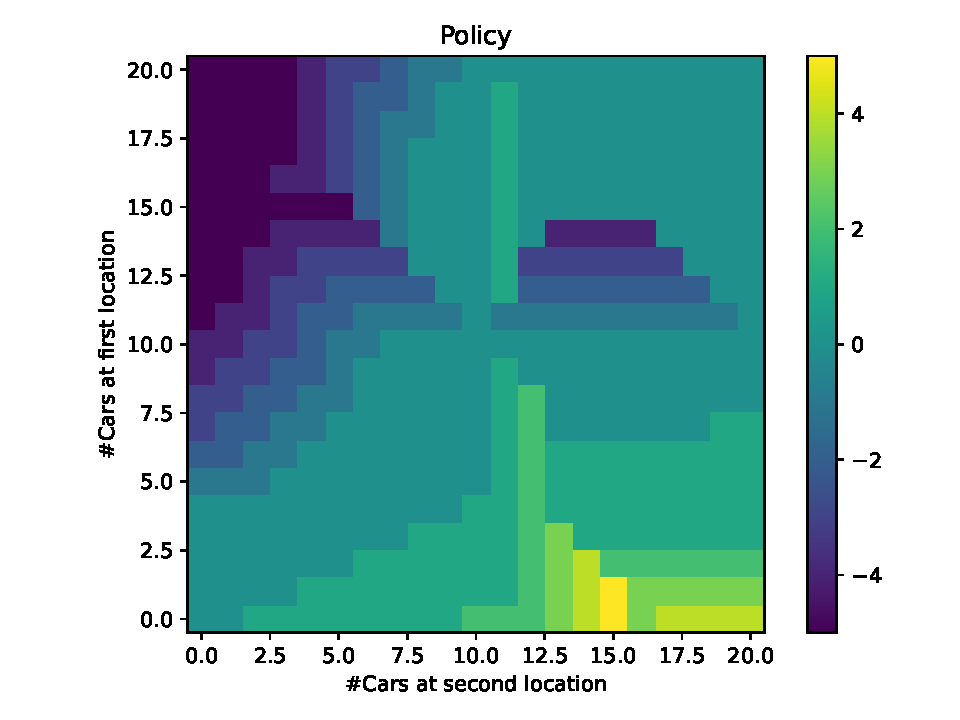
\includegraphics[width=0.8\textwidth]{chapters_latex/figures/ex_04_07_modified.pdf}
    \caption{The modified policy.}
\end{figure}

\subsection*{Exercise 4.8}
Why does the optimal policy for the gambler's problem have such a curious form? In particular, for capital of 50
it bets it all on one flip, but for capital of 51 it does not. Why is this a good policy? 

\subsubsection*{Solution:}

Betting 1 at 51 has two outcomes: receiving 1 coin with probability of 0.6 arriving at 52 coins, and losing 1 coin with probability of 0.4 arriving at 50 coins. At 50 coins we still have a relatively good chance of winning the game in one bet, and at 52 coins we have an even better chance. Betting more than one coin would mean that with great probability we would have less than 50 coins, in which case we would need a minimum of 2 bets to win the game, which is not good.

\subsection*{Exercise 4.9 (programming)}
Implement value iteration for the gambler's problem and
solve it for $p_h = 0.25$ and $p_h = 0.55$. In programming, you may find it convenient to
introduce two dummy states corresponding to termination with capital of 0 and 100,
giving them values of 0 and 1 respectively. Show your results graphically, as in Figure 4.3.
Are your results stable as $\theta \rightarrow 0$?

\subsubsection*{Solution:}

See the notebooks.

The state values for different head probabilities:

\begin{figure}[H]
    \centering
    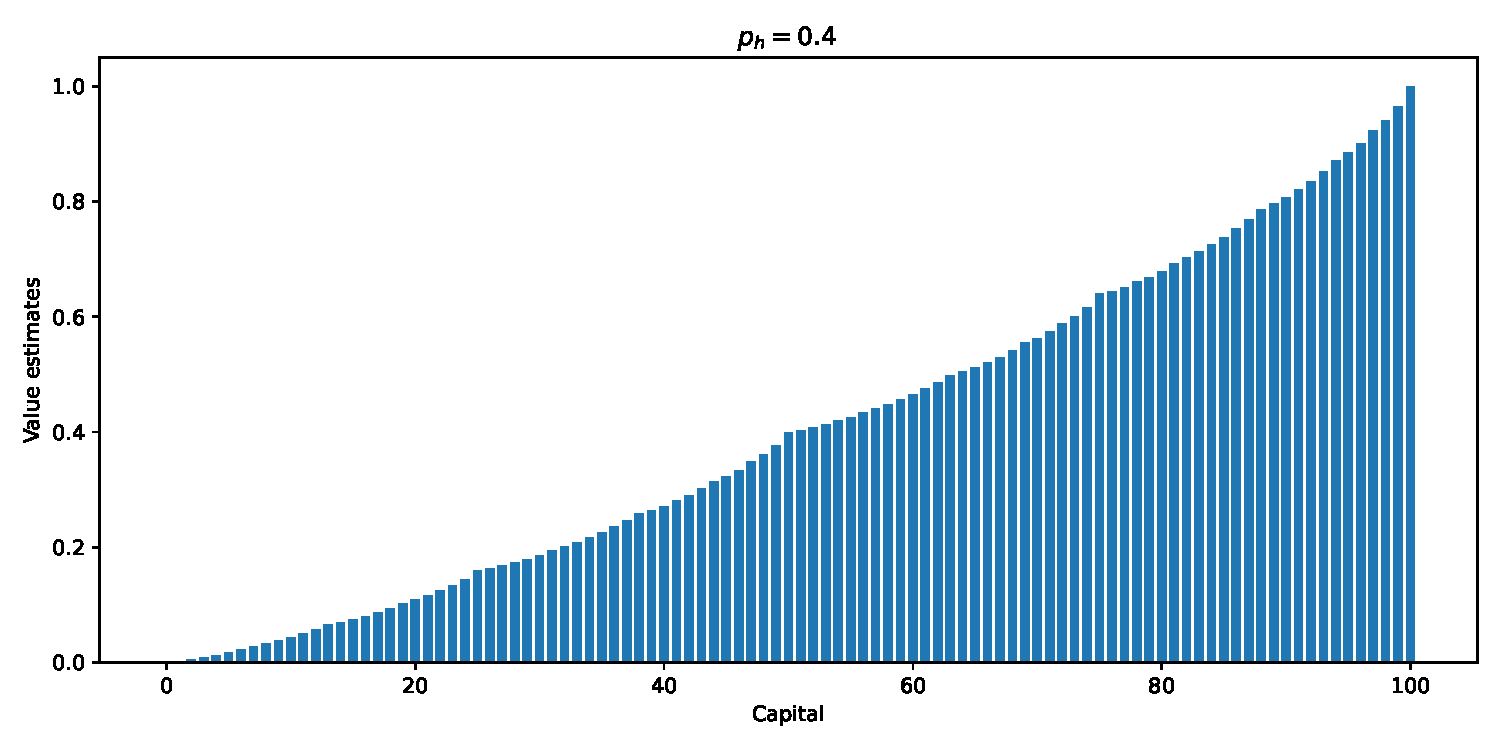
\includegraphics[width=0.8\textwidth]{chapters_latex/figures/ex_04_09_values_04.pdf}
\end{figure}

\begin{figure}[H]
    \centering
    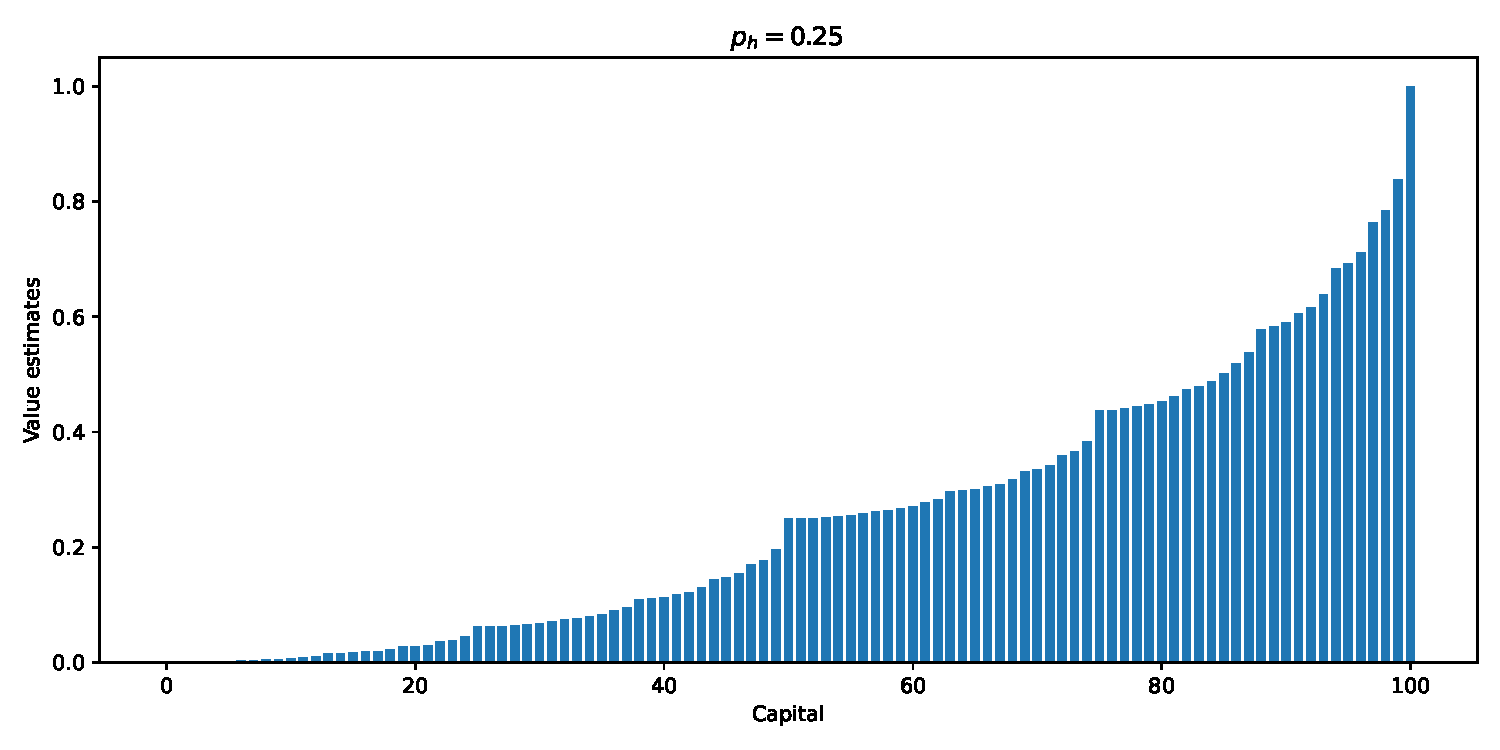
\includegraphics[width=0.8\textwidth]{chapters_latex/figures/ex_04_09_values_025.pdf}
\end{figure}

\begin{figure}[H]
    \centering
    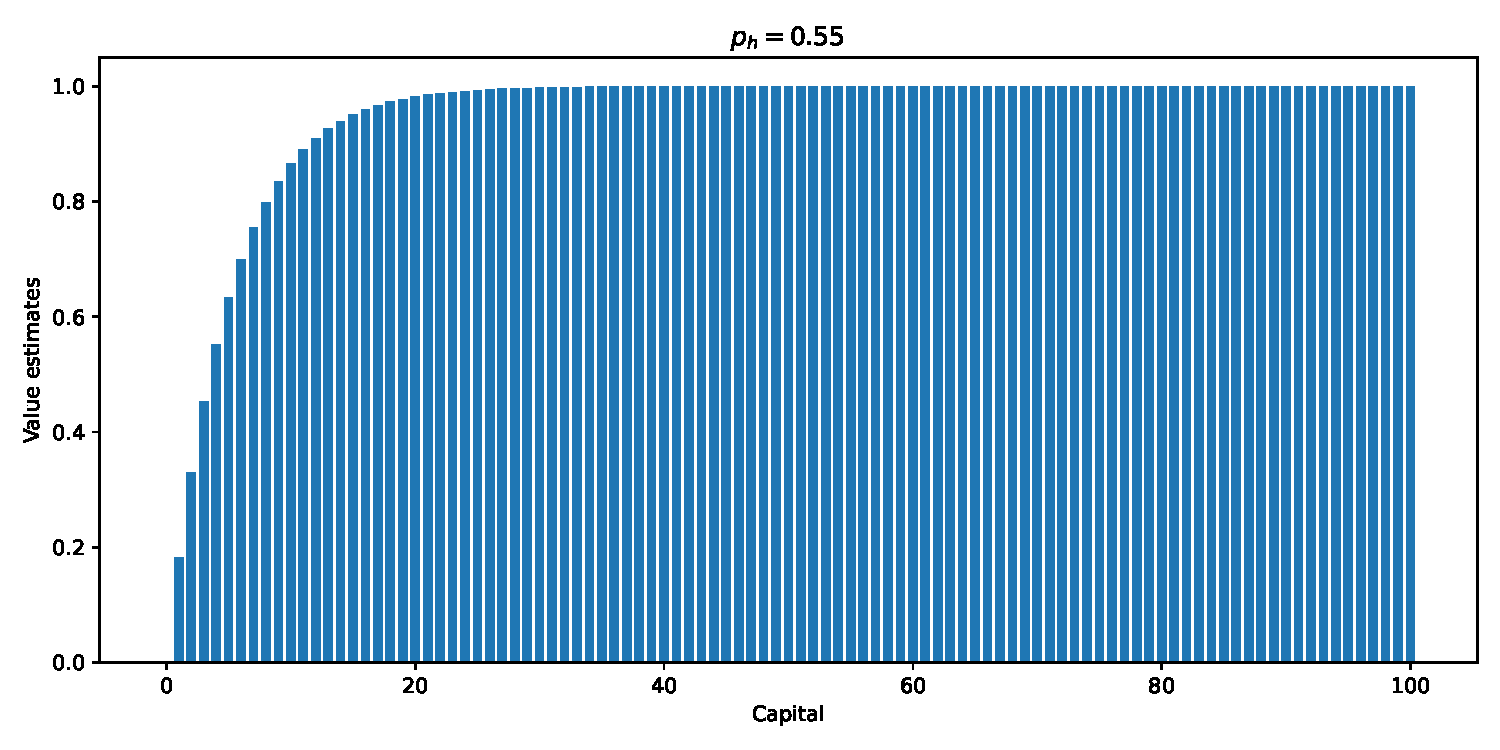
\includegraphics[width=0.8\textwidth]{chapters_latex/figures/ex_04_09_values_055.pdf}
\end{figure}

The optimal policies for different head probabilities:
\begin{figure}[H]
    \centering
    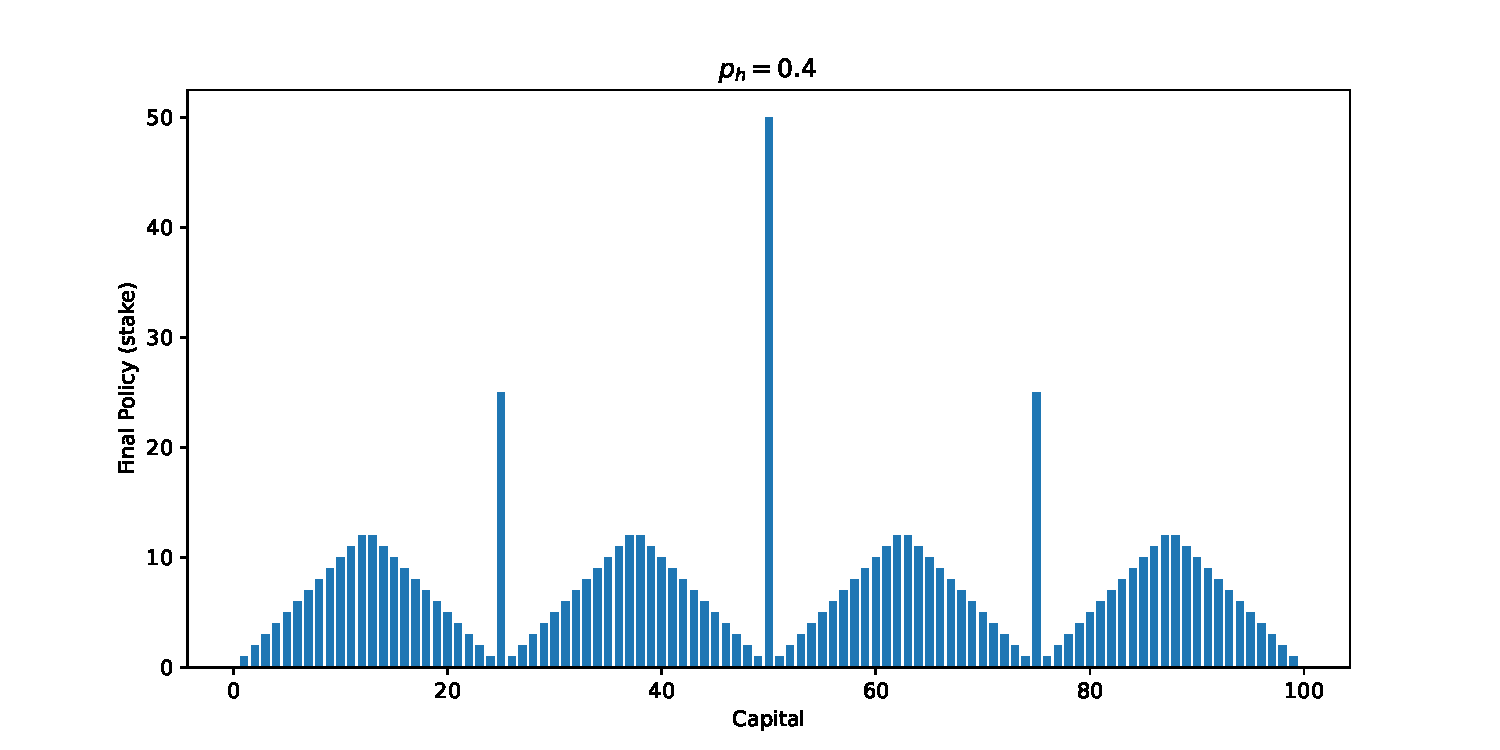
\includegraphics[width=0.8\textwidth]{chapters_latex/figures/ex_04_09_policies_04.pdf}
\end{figure}

\begin{figure}[H]
    \centering
    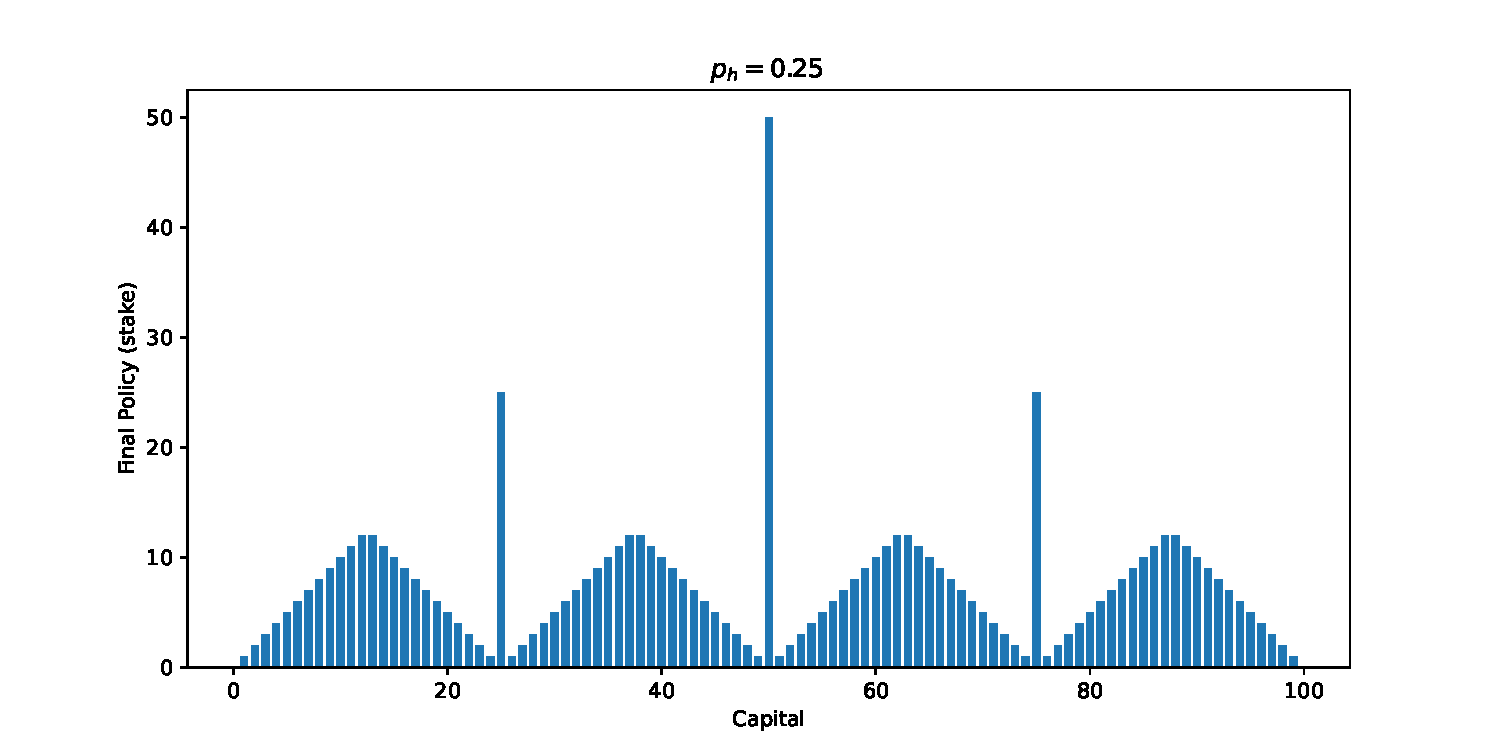
\includegraphics[width=0.8\textwidth]{chapters_latex/figures/ex_04_09_policies_025.pdf}
\end{figure}

\begin{figure}[H]
    \centering
    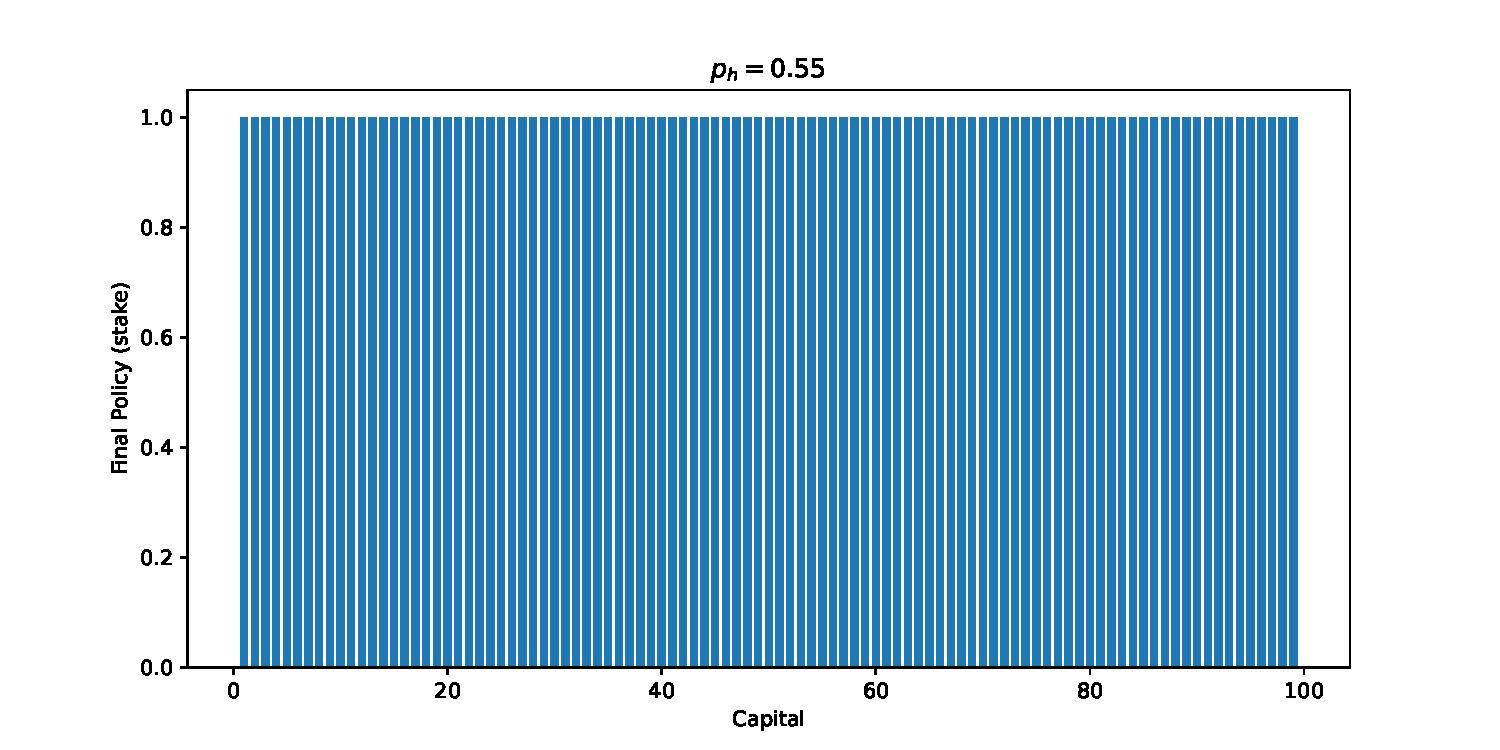
\includegraphics[width=0.8\textwidth]{chapters_latex/figures/ex_04_09_policies_055.pdf}
\end{figure}

\subsection*{Exercise 4.10}

What is the analog of the value iteration update (4.10) for action values,
$q_{k+1}(s,a)$?

\subsubsection*{Solution:}
\[
    q_{k+1}(s,a) = \sum_{s,r'} p(s',r \mid s, a) \left[r + \gamma \max_{a'} q_{k}(s',a') \right]
\]
\section*{Chapter 5}

\subsection*{Exercise 5.1}
Consider the diagrams on the right in Figure 5.1. Why does the estimated
value function jump up for the last two rows in the rear? Why does it drop off for the
whole last row on the left? Why are the frontmost values higher in the upper diagrams
than in the lower?

\subsubsection*{Solution:}

The estimated value function jumps up for the last two rows in the rear because the player has a high probability of winning at 20 and 21, as the dealer is likely to have lower value or go bust.

It drops off for the whole last row on the left because having an ace is a big advantage, thus if the dealer has an ace the probability of the player winning is less.

The frontmost values are higher in the upper diagrams than in the lower because having an usable ace gives an advantage, as the probability of going bust on the next draw is less.

\subsection*{Exercise 5.2}
Suppose every-visit MC was used instead of first-visit MC on the blackjack
task. Would you expect the results to be very different? Why or why not?

\subsubsection*{Solution:}
It would be similar, as in an episode the probability of visiting the same state twice is very low, so the end results would be almost identical. One such rare case is having two aces, then getting a 10.

\subsection*{Exercise 5.3}
What is the backup diagram for Monte Carlo estimation of $q_\pi$? 

\subsubsection*{Solution:}

\begin{figure}[H]
    \centering
    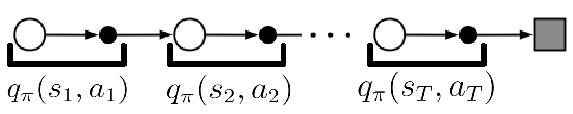
\includegraphics[width=0.8\textwidth]{chapters_latex/figures/ex_05_03.png}
\end{figure}


\subsection*{Exercise 5.4}
The pseudocode for Monte Carlo ES is inefficient because, for each state-
action pair, it maintains a list of all returns and repeatedly calculates their mean. It would
be more efficient to use techniques similar to those explained in Section 2.4 to maintain
just the mean and a count (for each state-action pair) and update them incrementally.
Describe how the pseudocode would be altered to achieve this.

\subsubsection*{Solution:}
We would need to initialize a counter variable $N(s,a) = 0 \quad \forall s \in S, \forall a \in A$, we don't need $\text{Returns}(s,a)$ and $Q(s,a)=0 \quad \forall s \in S, \forall a \in A$. 
In the last step we should have the following:
\begin{itemize}
    \item[] $N(S_t, A_t) \leftarrow N(S_t, A_t) + 1$
    \item[] $Q(S_t, A_t) \leftarrow Q(S_t, A_t) + (G - Q(S_t, A_t))/N(S_t, A_t)$
\end{itemize}

\subsection*{Exercise 5.5}
Consider an MDP with a single nonterminal state and a single action
that transitions back to the nonterminal state with probability $p$ and transitions to the
terminal state with probability $1-p$. Let the reward be $+1$ on all transitions, and let
$\gamma = 1$. Suppose you observe one episode that lasts 10 steps, with a return of 10. What
are the first-visit and every-visit estimators of the value of the nonterminal state?

\subsubsection*{Solution:}
First visit:
\[
    V(S) = 10
\]

Every visit:

\[
    V(S) = \frac{10 + 9 + \dots + 1}{10} = 5.5
\]

\subsection*{Exercise 5.6}
What is the equation analogous to (5.6) for $\textit{action}$ values $Q(s, a)$ instead of
state values $V(s)$, again given returns generated using $b$?

\subsubsection*{Solution:}
\[
    Q(s,a) = \frac{\sum_{t \in \mathcal{T}(s,a)} \rho_{t+1:T(t)-1} G_t}{\sum_{t \in \mathcal{T}(s,a)} \rho_{t+1:T(t)-1}}
\]
 
Where $\mathcal{T}(s,a)$ are the timesteps where action $a$ was takein in state $s$.


\subsection*{Exercise 5.7}
In learning curves such as those shown in Figure 5.3 error generally decreases
with training, as indeed happened for the ordinary importance-sampling method. But for
the weighted importance-sampling method error first increased and then decreased. Why
do you think this happened? 

\subsubsection*{Solution:}

In the beginning there are no good samples, so the estimate is 0. After the first usable sample the estimate might be -1, 0 or 1. This increases the MSE of a single run. In the first 10 episodes more and more runs get their first usable samples, so on average the MSE also increases.

\subsection*{Exercise 5.8}
The results with Example 5.5 and shown in Figure 5.4 used a first-visit MC
method. Suppose that instead an every-visit MC method was used on the same problem.
Would the variance of the estimator still be infinite? Why or why not? 

\subsubsection*{Solution:}

Yes, it would still be infinite. Following the proof in the book, instead of at length $n$ only considering that episode consisting of $n$ timesteps, we should take average of all subsamples in that episode. As the importance of the last timestep is the least, this average is greater than the value in first-visit example.


\subsection*{Exercise 5.9}
Modify the algorithm for first-visit MC policy evaluation (Section 5.1) to
use the incremental implementation for sample averages described in Section 2.4.

\subsubsection*{Solution:}
\fbox{
\begin{minipage}{0.95\textwidth}
\footnotesize
Input: a policy $\pi$ to be evaluated \\
Initialize:
\begin{itemize}
    \item[] $V(s) \leftarrow 0$, for all $s \in S$
    \item[] $N(s) \leftarrow 0$, for all $s \in S$
\end{itemize}

Loop forever (for each episode):
\begin{itemize}
    \item[] Generate an episode following $\pi$: $S_0, A_0, R_1, S_1, A_1, R_2, \ldots, S_{T-1}, A_{T-1}, R_T$
    \item[] $G \leftarrow 0$
    \item[] Loop for each step of episode, $t = T-1, T-2, \ldots, 0$:
    \begin{itemize}
        \item[] $G \leftarrow \gamma G + R_{t+1}$
        \item[] Unless $S_t$ appears in $S_0, S_1, \ldots, S_{t-1}$:
        \begin{itemize}
            \item[] $N(s) \leftarrow N(s) + 1$
            \item[] $V(S_t) \leftarrow V(S_t) + (G - V(S_t))/N(S_t)$
        \end{itemize}
    \end{itemize}
\end{itemize}
\end{minipage}
}


\subsection*{Exercise 5.10}
Derive the weighted-average update rule (5.8) from (5.7). Follow the pattern of the derivation of the unweighted rule (2.3).

\subsubsection*{Solution:}

\begin{align*}
    V_{n+1} &= \frac{\sum_{k=1}^{n}W_k G_k}{\sum_{k=1}^{n}W_k} \\
    &= \frac{W_{n}G_{n} + \sum_{k=1}^{n-1}W_k G_k}{C_n} \\
    &= \frac{W_{n}G_{n} + V_{n}(C_{n}-W_n)}{C_{n}} \\
    &= V_n + \frac{W_n}{C_n}\left[ G_n - V_n\right]
\end{align*}


\subsection*{Exercise 5.11}
In the boxed algorithm for off-policy MC control, you may have been
expecting the W update to have involved the importance-sampling ratio $\frac{\pi(A_t \mid S_t)}{b(A_t \mid S_t)}$, but
instead it involves $\frac{1}{b(A_t \mid S_t)}$. Why is this nevertheless correct?

\subsubsection*{Solution:}

The policy $\pi$ is greedy, it always chooses the action it thinks is best with probability 1, so  $\pi(A_t \mid S_t) = 1$.


\subsection*{Exercise 5.11: Racetrack (programming)}
Consider driving a race car around a turn
like those shown in Figure 5.5. You want to go as fast as possible, but not so fast as
to run off the track. In our simplified racetrack, the car is at one of a discrete set of
grid positions, the cells in the diagram. The velocity is also discrete, a number of grid
cells moved horizontally and vertically per time step. The actions are increments to the
velocity components. Each may be changed by +1, $-1$, or 0 in each step, for a total of
nine $(3 \times 3)$ actions. Both velocity components are restricted to be nonnegative and less
than 5, and they cannot both be zero except at the starting line. Each episode begins
in one of the randomly selected start states with both velocity components zero and
ends when the car crosses the finish line. The rewards are -1 for each step until the car
crosses the finish line. If the car hits the track boundary, it is moved back to a random
position on the starting line, both velocity components are reduced to zero, and the
episode continues. Before updating the car's location at each time step, check to see if
the projected path of the car intersects the track boundary. If it intersects the finish line,
the episode ends; if it intersects anywhere else, the car is considered to have hit the track
boundary and is sent back to the starting line. To make the task more challenging, with
probability 0.1 at each time step the velocity increments are both zero, independently of
the intended increments. Apply a Monte Carlo control method to this task to compute
the optimal policy from each starting state. Exhibit several trajectories following the
optimal policy (but turn the noise off for these trajectories).

\subsubsection*{Solution:}

See the notebooks.

\begin{figure}[H]
    \centering
    \begin{minipage}[b]{0.35\textwidth}
      \centering
      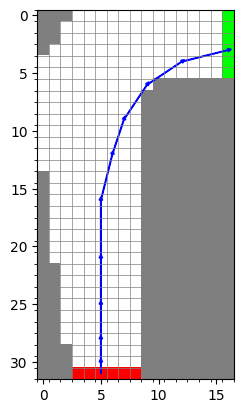
\includegraphics[width=\textwidth]{chapters_latex/figures/ex_05_12_1.png}
      
    \end{minipage}
    \hspace{0.05\textwidth} % Adjusts the horizontal space between images
    \begin{minipage}[b]{0.45\textwidth}
      \centering
      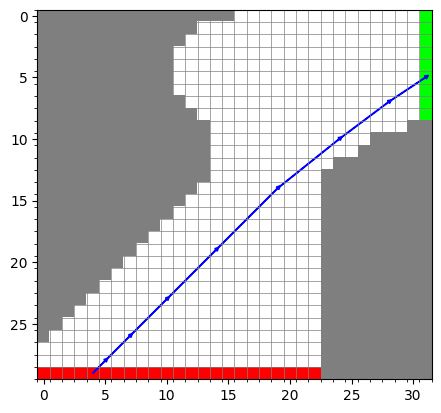
\includegraphics[width=\textwidth]{chapters_latex/figures/ex_05_12_2.png}
    \end{minipage}
  \end{figure}

\subsection*{*Exercise 5.13}
Show the steps to derive (5.14) from (5.12).

\subsubsection*{Solution:}

\begin{multline*}
    \mathbb{E} \left[ \rho_{t:T-1} R_{t+1} \right] = \mathbb{E} \left[ \prod_{k=t}^{T-1} \frac{\pi(A_k \mid S_t)}{b(A_k \mid S_k)} R_{t+1} \right] \\
    = \sum_{A, S, R} \left(\prod_{k=t}^{T-1}\left( p(S_{k+1}, R_{k+1}\mid S_k, A_k) b(A_k \mid S_t) \right) \prod_{k=t}^{T-1} \frac{\pi(A_k \mid S_k)}{b(A_k \mid S_k)} R_{t+1} \right) \\
    = \sum_{A, S, R} \left(\prod_{k=t}^{T-1}\left( p(S_{k+1}, R_{k+1}\mid S_k, A_k) \right) \prod_{k=t}^{T-1} \pi(A_k \mid S_k) R_{t+1} \right) \\
    = \sum_{A, S, R} \left(  R_{t+1} \prod_{k=t}^{T-1}\left( p(S_{k+1}, R_{k+1}\mid S_k, A_k) \right) \prod_{k=t}^{T-1} \pi(A_k \mid S_k) \right) \\
    = \sum_{A_t, S_t, R_{t+1}}   R_{t+1} p(S_{k+1}, R_{t+1}\mid S_t, A_t) \pi(A_t \mid S_t) \\
    = \sum_{A_t, S_t, R_{t+1}}   R_{t+1} p(S_{k+1}, R_{t+1}\mid S_t, A_t) \frac{\pi(A_t \mid S_t)}{b(A_t \mid S_t)} b(A_t \mid S_t)\\
    = \mathbb{E} \left[ \rho_{t:t} R_{t+1} \right] \\
\end{multline*} 


\subsection*{*Exercise 5.14}
Modify the algorithm for off-policy Monte Carlo control (page 111) to use
the idea of the truncated weighted-average estimator (5.10). Note that you will first need
to convert this equation to action values. 

\subsubsection*{Solution:}
We want to achieve this:
\footnotesize
\begin{align*}
Q(s,a) &= \frac{\sum_{t \in \mathcal{T}(s,a)} \left( (1 - \gamma) \textcolor{red}{\sum_{h = t+1}^{T(t) - 1} \gamma^{h - t - 1} \rho_{t:h-1} \bar{G}_{t:h}} + \textcolor{blue}{\gamma^{T(t) - t - 1} \rho_{t:T(t) - 1}} \bar{G}_{t:T(t)} \right)}
{\sum_{t \in \mathcal{T}(s,a)} \left( (1 - \gamma) \textcolor{green}{\sum_{h = t+1}^{T(t) - 1} \gamma^{h - t - 1} \rho_{t:h-1}} + \textcolor{blue}{\gamma^{T(t) - t - 1} \rho_{t:T(t) - 1}} \right)} \\
    &= \frac{\sum_{t \in \mathcal{T}(s,a)} \left( (1 - \gamma) \textcolor{red}{A_t} + \textcolor{blue}{W_t} \bar{G}_{t:T(t)} \right)}
{\sum_{t \in \mathcal{T}(s,a)} \left( (1 - \gamma) \textcolor{green}{B_t} + \textcolor{blue}{W_t} \right)}
\end{align*}

\[
    W_{t-1} = W_t \gamma \frac{1}{b(A_{t-1} \mid S_{t-1})}
\]

\[
    B_{t-1} = (\gamma B_t + 1) \frac{1}{b(A_{t-1} \mid S_{t-1})}
\]

\[
    A_{t-1} = (\gamma A_t + R_{t}) \frac{1}{b(A_{t-1} \mid S_{t-1})} + R_{t-1} B_{t-1}
\]

\fbox{
\begin{minipage}{0.95\textwidth}
\footnotesize
Initialize, for all $s \in S$, $a \in A(s)$:
\begin{itemize}
    \item[] $Q(s, a) \in \mathbb{R}$ (arbitrarily)
    \item[] $C(s, a) \leftarrow 0$
    \item[] $\pi(s) \leftarrow \arg \max_a Q(s, a)$ \hspace{10pt} (with ties broken consistently)
\end{itemize}

Loop forever (for each episode):
\begin{itemize}
    \item[] $b \leftarrow$ any soft policy
    \item[] Generate an episode using $b$: $S_0, A_0, R_1, \ldots, S_{T-1}, A_{T-1}, R_T$
    \item[] $\bar{G} \leftarrow R_T$
    \item[] $W \leftarrow \frac{1}{b(A_{T-1} \mid S_{T-1})}$
    \item[] $A \leftarrow 0$
    \item[] $B \leftarrow 0$
    \item[] Loop for each step of episode, $t = T-1, T-2, \ldots, 0$:
    \begin{itemize}
        \item[] $C(S_t, A_t) \leftarrow C(S_t, A_t) + (1-\gamma)B + W$
        \item[] $Q(S_t, A_t) \leftarrow Q(S_t, A_t) + \frac{(1-\gamma)B + W}{C(S_t, A_t)} [(1-\gamma)A + W \bar{G} - Q(S_t, A_t)]$
        \item[] $\bar{G} \leftarrow \bar{G} + R_{t}$
        \item[] $W \leftarrow W \gamma \frac{1}{b(A_{t-1} \mid S_{t-1})}$
        \item[] $B \leftarrow (\gamma B + 1) \frac{1}{b(A_t \mid S_t)}$
        \item[] $A \leftarrow (\gamma A + R_t)\frac{1}{b(A_t \mid S_t)} + R_{t-1}B $
        \item[] $\pi(S_t) \leftarrow \arg \max_a Q(S_t, a)$ \hspace{10pt} (with ties broken consistently)
        \item[] If $A_t \neq \pi(S_t)$ then exit inner Loop (proceed to next episode)
        
    \end{itemize}
\end{itemize}
\end{minipage}
}


\subsection*{Exercise 5.15}
Make new equations analogous to the importance-sampling Monte Carlo
estimates (5.5) and (5.6), but for action value estimates $Q(s, a)$. You will need new
notation $\mathcal{T}(s,a)$ for the time steps on which the state-action pair $s$, $a$ is visited on the
episode. Do these estimates involve more or less importance-sampling correction?

\subsubsection*{Solution:}

\[
Q(s,a) = \frac{\sum_{t \in \mathcal{T}(s,a)} \rho_{t+1:T(t) - 1} G_t}
{|\mathcal{T}(s,a)|}
\]

\[
Q(s,a) = \frac{\sum_{t \in \mathcal{T}(s,a)} \rho_{t+1:T(t) - 1} G_t}
{\sum_{t \in \mathcal{T}(s,a)} \rho_{t+1:T(t) - 1}}
\]

They involve less importance sampling correction, as we are not including $\frac{\pi(a \mid s)}{b(a \mid s)}$ in the equation. $\pi(a \mid s)$ can even be 0 in which case the result would be always 0 or undefined which is not right.
\section*{Chapter 6}

\subsection*{Exercise 6.1}
If $V$ changes during the episode, then (6.6) only holds approximately; what
would the difference be between the two sides? Let $V_t$ denote the array of state values
used at time $t$ in the TD error (6.5) and in the TD update (6.2). Redo the derivation
above to determine the additional amount that must be added to the sum of TD errors
in order to equal the Monte Carlo error. 

\subsubsection*{Solution:}

\begin{align*}
G_t - V(S_t) &= R_{t+1} + \gamma G_{t+1} - V_t(S_t) + \gamma V_{t}(S_{t+1}) - \gamma V_{t}(S_{t+1}) \\
&= \delta_t + \gamma G_{t+1} - \gamma V_t(S_{t+1}) \\
&= \delta_t + \gamma R_{t+2} + \gamma^2 G_{t+2} - \gamma V_{t}(S_{t+1}) \\
&= \delta_t + \gamma (R_{t+2} + \gamma V_{t+1}(S_{t+2}) - V_{t+1}(S_{t+1}) - \gamma V_{t+1}(S_{t+2}) + V_{t+1}(S_{t+1}))\\
& \quad + \gamma^2 G_{t+2} - \gamma V_{t}(S_{t+1}) \\
&= \delta_t + \gamma \delta_{t+1} - \gamma^2 V_{t+1}(S_{t+2}) + \gamma V_{t+1}(S_{t+1}) + \gamma^2 G_{t+2} - \gamma V_{t}(S_{t+1})\\
& \dots \\
&= \sum_{k=t}^{T-1} \gamma^{k-t} \delta_k + \sum_{k=t+1}^{T-1} \gamma^{k-t } \left[V_{k}(S_{k}) - V_{k-1}(S_{k}) \right]
\end{align*}


\subsection*{Exercise 6.2}
This is an exercise to help develop your intuition about why TD methods
are often more efficient than Monte Carlo methods. Consider the driving home example
and how it is addressed by TD and Monte Carlo methods. Can you imagine a scenario
in which a TD update would be better on average than a Monte Carlo update? Give
an example scenario — a description of past experience and a current state—in which
you would expect the TD update to be better. Here's a hint: Suppose you have lots
of experience driving home from work. Then you move to a new building and a new
parking lot (but you still enter the highway at the same place). Now you are starting
to learn predictions for the new building. Can you see why TD updates are likely to be
much better, at least initially, in this case? Might the same sort of thing happen in the
original scenario?

\subsubsection*{Solution:}

In the example scenario, after moving to a new building and a new parking lot, the agent still enters the highway at the same place. 
The agent has a lot of experience driving home from work, so it has a good estimate of the value of the state of entering the highway.
However, the agent has no experience with the new building and parking lot, so the Monte Carlo update would require the agent to drive
home from work many times to get a good estimate of the value of the state of the new building and parking lot. On the other hand, the
TD update would only require the agent to drive home from work once (or twice) to get a good estimate of the value of the state of the parking lot
and new building. Therefore, the TD update would be better in this case.


\subsection*{Exercise 6.3}
From the results shown in the left graph of the random walk example it
appears that the first episode results in a change in only V(A). What does this tell you
about what happened on the first episode? Why was only the estimate for this one state
changed? By exactly how much was it changed? 

\subsubsection*{Solution:}
It tells us that the first episode ended on the left side of the random walk.
The update equation:
\[
V(S_t) \leftarrow V(S_t) + \alpha \left[R_{t+1} + \gamma V(S_{t+1}) - V(S_t)\right]
\]

$\gamma = 1$, $\alpha = 0.1$, $V(A) = 0.5$, $V(B) = 0.5$, $V(C) = 0.5$, $V(D) = 0.5$, $V(E) = 0.5$.

While the agent receives a reward of 0, the following happens:

\[
V(S_t) \leftarrow 0.5 + 0.1 \left[0 + 1 \cdot 0.5 - 0.5\right] = 0.5
\]

After the agent chose to go left at state $A$, with $V(\text{terminal state}) = 0$:
\[
V(A) \leftarrow 0.5 + 0.1 \left[0 + 1 \cdot 0 - 0.5\right] = 0.45
\]


\subsection*{Exercise 6.4}
The specific results shown in the right graph of the random walk example
are dependent on the value of the step-size parameter, $\alpha$. Do you think the conclusions
about which algorithm is better would be affected if a wider range of $\alpha$ values were used?
Is there a different, fixed value of $\alpha$ at which either algorithm would have performed
significantly better than shown? Why or why not?

\subsubsection*{Solution:}
Using different values of $\alpha$ would not affect the conclusions about which algorithm is better.
If $\alpha$ would be smaller, the algorithms would converge slower, but would approximate the true value function better.
If $\alpha$ would be larger, the algorithms would converge faster, but would approximate the true value function worse, as we are more dependent on the more recently observed rewards.

\subsection*{*Exercise 6.5}
In the right graph of the random walk example, the RMS error of the
TD method seems to go down and then up again, particularly at high $\alpha$'s. What could
have caused this? Do you think this always occurs, or might it be a function of how the
approximate value function was initialized? 

\subsubsection*{Solution:}
The increase in RMS error for TD at high $\alpha$ values is due to instability and overshooting caused by 
large step sizes, leading to divergence from the true values. While initialization can affect early learning dynamics,
it does not prevent this instability at high $\alpha$.

\subsection*{Exercise 6.6}
In Example 6.2 we stated that the true values for the random walk example
are $\frac{1}{6}, \frac{2}{6}, \frac{3}{6}, \frac{4}{6}$, and $\frac{5}{6}$ for states A through E. Describe at least two different ways that
these could have been computed. Which would you guess we actually used? Why?

\subsubsection*{Solution:}

We could write this as a system of linear equations:
\[
\begin{bmatrix}
    0 & 0.5 & 0 & 0 & 0 \\
    0.5 & 0 & 0.5 & 0 & 0 \\
    0 & 0.5 & 0 & 0.5 & 0 \\
    0 & 0 & 0.5 & 0 & 0.5 \\
    0 & 0 & 0 & 0.5 & 0 
\end{bmatrix}
\begin{bmatrix}
    V(A) \\
    V(B) \\
    V(C) \\
    V(D) \\
    V(E) 
\end{bmatrix}
+
\begin{bmatrix}
    0 \\
    0 \\
    0 \\
    0 \\
    0.5
\end{bmatrix}
=
\begin{bmatrix}
    V(A) \\
    V(B) \\
    V(C) \\
    V(D) \\
    V(E) 
\end{bmatrix}
\]

\[
    \begin{bmatrix}
        -1 & 0.5 & 0 & 0 & 0 \\
        0.5 & -1 & 0.5 & 0 & 0 \\
        0 & 0.5 & -1 & 0.5 & 0 \\
        0 & 0 & 0.5 & -1 & 0.5 \\
        0 & 0 & 0 & 0.5 & -1 
    \end{bmatrix}
    \begin{bmatrix}
        V(A) \\
        V(B) \\
        V(C) \\
        V(D) \\
        V(E) 
    \end{bmatrix}
    =
    \begin{bmatrix}
        0 \\
        0 \\
        0 \\
        0 \\
        -0.5
    \end{bmatrix}
\]

\[
    \begin{bmatrix}
        V(A) \\
        V(B) \\
        V(C) \\
        V(D) \\
        V(E) 
    \end{bmatrix}
    =
    \begin{bmatrix}
        1/6 \\
        2/6 \\
        3/6 \\
        4/6 \\
        5/6
    \end{bmatrix}
\]

Or we could also solve this problem with the dynamic programming approach. I think this way used, as it is relevant to the context of the book.

\subsection*{*Exercise 6.7}
Design an off-policy version of the TD(0) update that can be used with
arbitrary target policy $\pi$ and covering behavior policy $b$, using at each step $t$ the importance
sampling ratio $\rho_{t:t}$ (5.3).

\subsubsection*{Solution:}

\begin{align*}
    V(S_t) &= \mathbb{E}_\pi[G_t \mid S_t = s] \\
    &= \sum_{a} \pi(a \mid s) \sum_{s', r} p(s', r \mid s, a) \left[ r + \gamma V(s') \right] = \\
    &= \sum_{a} b(a \mid s) \sum_{s', r} p(s', r \mid s, a) \frac{\pi(a \mid s)}{b(a \mid s)} \left[ r + \gamma V(s') \right] \left[ r' + \gamma V(s'') \right] \\
    &= \mathbb{E}_b[\rho_{t:t} G_t \mid S_t = s] = \mathbb{E}_b[\rho_{t:t} (R_{t+1} + \gamma V(S_{t+1})) \mid S_t = s]
\end{align*}


\[
V(S_t) \leftarrow V(S_t) + \alpha  \left[ \rho_{t:t}(R_{t+1} + \gamma V(S_{t+1})) - V(S_t) \right]
\]

\subsection*{Exercise 6.8}
Show that an action-value version of (6.6) holds for the action-value form
of the TD error  $\delta_t = R_{t+1} + \gamma Q(S_{t+1}, A_{t+1}) - Q(S_t, A_t)$, again assuming that the values
don't change from step to step. 

\subsubsection*{Solution:}

\begin{align*}
    G_t - Q(S_t, A_t) &= R_{t+1} + \gamma G_{t+1} - Q(S_t, A_t) + \gamma Q(S_{t+1}, A_{t+1}) - \gamma Q(S_{t+1}, A_{t+1}) \\
    &= \delta_t + \gamma (G_{t+1} - Q(S_{t+1}, A_{t+1})) \\
    &= \delta_t + \gamma \delta_{t+1} + \gamma^2 (G_{t+2} - Q(S_{t+1}, A_{t+2})) \\
    &= \delta_t + \gamma \delta_{t+1} + \gamma^2 \delta_{t+2} + \cdots + \gamma^{T-t-1} \delta_{T-1} + \gamma^{T-t} (G_T - Q(S_{T}, A_{T})) \\
    &= \delta_t + \gamma \delta_{t+1} + \gamma^2 \delta_{t+2} + \cdots + \gamma^{T-t-1} \delta_{T-1} + \gamma^{T-t} (0 - 0) \\
    &= \sum_{k=t}^{T-1} \gamma^{k-t} \delta_k.
\end{align*}


\subsection*{Exercise 6.9: Windy Gridworld with King's Moves (programming)}
Re-solve the windy gridworld assuming eight possible actions, including the diagonal moves, rather than four.
How much better can you do with the extra actions? Can you do even better by including
a ninth action that causes no movement at all other than that caused by the wind?

\subsubsection*{Solution:}
See the notebook.
\begin{figure}[H]
    \centering
    \begin{minipage}[b]{0.47\textwidth}
      \centering
      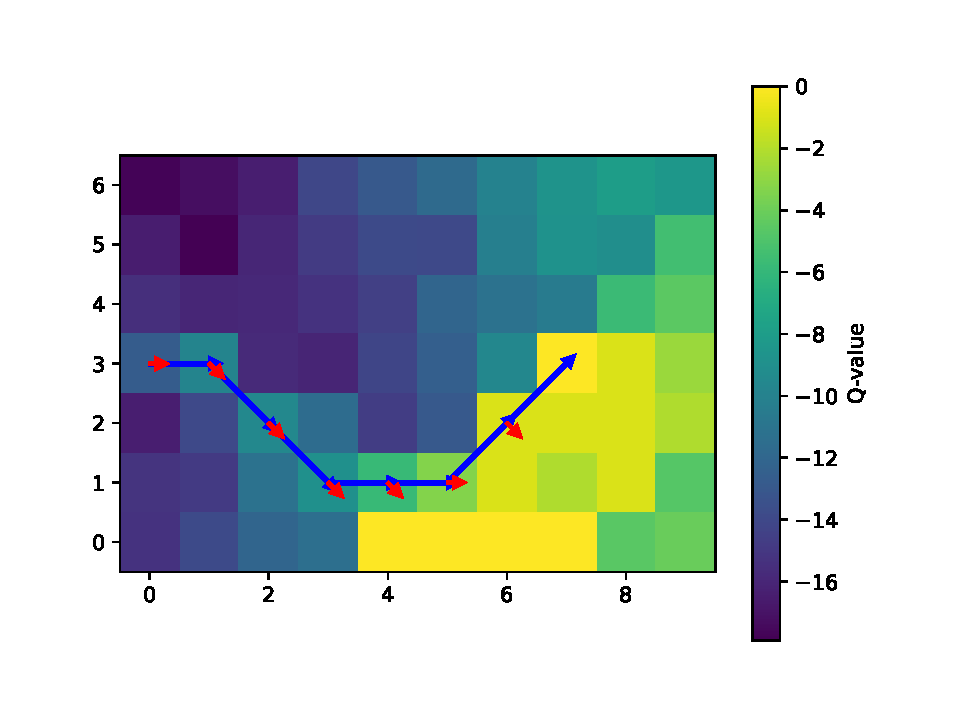
\includegraphics[width=\textwidth]{chapters_latex/figures/ex_06_09_king_moves.pdf}
      \captionsetup{labelformat=empty}
      \caption{King's Moves}
      
    \end{minipage}
    \hspace{0.04\textwidth} % Adjusts the horizontal space between images
    \begin{minipage}[b]{0.47\textwidth}
        \centering
        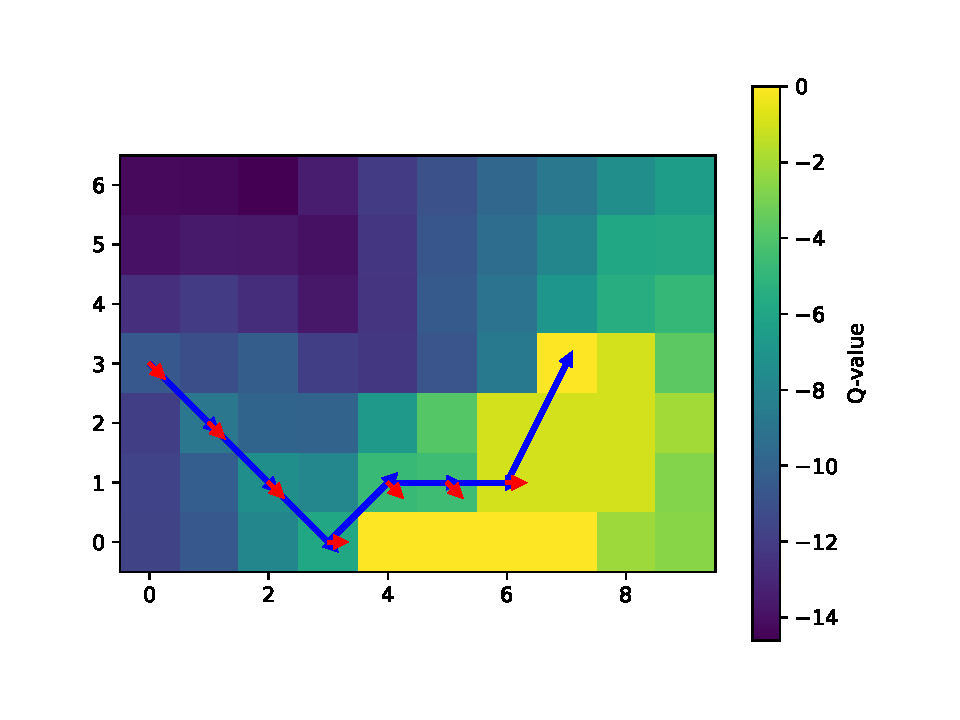
\includegraphics[width=\textwidth]{chapters_latex/figures/ex_06_09_king_moves_plus_zero.pdf}
        \captionsetup{labelformat=empty}
        \caption{King's Moves and Zero Action}
    \end{minipage}
  \end{figure}

\subsection*{Exercise 6.10: Stochastic Wind (programming)}
Re-solve the windy gridworld task with
King's moves, assuming that the effect of the wind, if there is any, is stochastic, sometimes
varying by 1 from the mean values given for each column. That is, a third of the time
you move exactly according to these values, as in the previous exercise, but also a third
of the time you move one cell above that, and another third of the time you move one
cell below that. For example, if you are one cell to the right of the goal and you move
left , then one-third of the time you move one cell above the goal, one-third of the time
you move two cells above the goal, and one-third of the time you move to the goal.

\subsubsection*{Solution:}
See the notebook.
\begin{figure}[H]
    \centering
    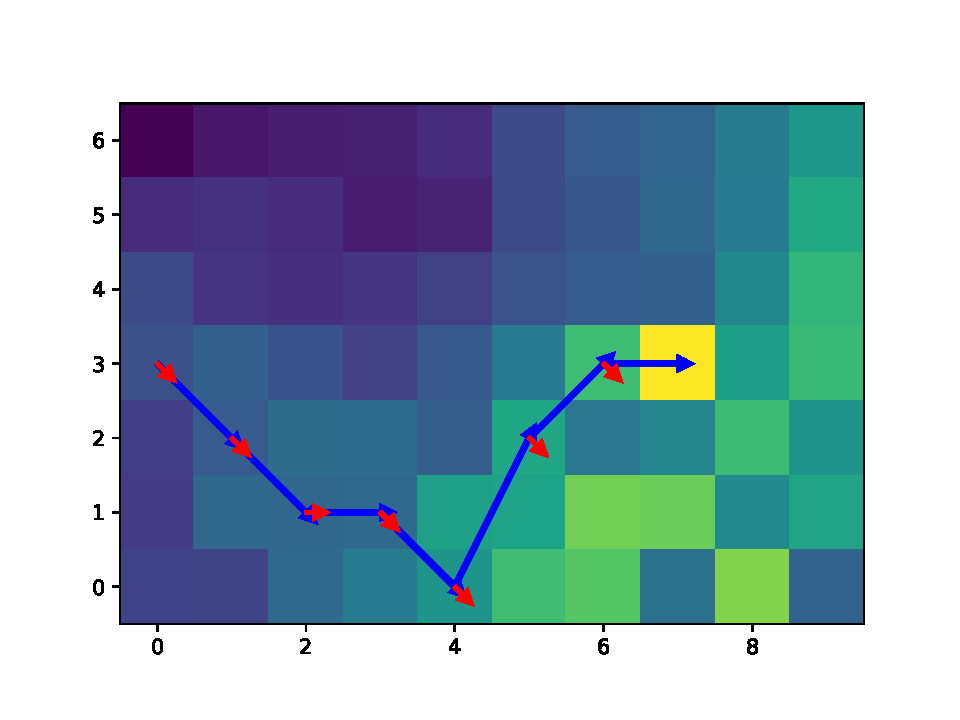
\includegraphics[width=0.65\textwidth]{chapters_latex/figures/ex_06_10.pdf}
    \captionsetup{labelformat=empty}
    \caption{King's Moves and Stochastic Wind}
\end{figure}

The average number of steps to reach the goal is 13.449 in my implementation, this could be improved by tuning the hyperparameters ($\varepsilon$, $\alpha$) and the number of episodes.

\subsection*{Exercise 6.11}
Why is Q-learning considered an off-policy control method?

\subsubsection*{Solution:}
Q-learning is an off-policy method because it learns the optimal policy independently of the
agent's current behavior policy by updating Q-values based on the maximum possible future reward, not the action actually taken.

\subsection*{Exercise 6.12}
Suppose action selection is greedy. Is Q-learning then exactly the same
algorithm as Sarsa? Will they make exactly the same action selections and weight
updates?

\subsubsection*{Solution:}
If action selection is greedy for both Q-learning and SARSA, is can be said that they are the same algorithm. 

The update for Q-learning:
\[
Q(s, a) \leftarrow Q(s, a) + \alpha \left( r + \gamma \max_{a'} Q(s', a') - Q(s, a) \right)
\]

The update for SARSA:
\[
Q(s, a) \leftarrow Q(s, a) + \alpha \left( r + \gamma Q(s', a') - Q(s, a) \right)
\]
Where $Q(s', a') = \max_{a'} Q(s', a')$

These are the same, so the updates are equal for the same $s$ and $a$.

Since both algorithms have the same policy, they will make the same action selections too.


\subsection*{*Exercise 6.13}
What are the update equations for Double Expected Sarsa with an
$\varepsilon$-greedy target policy?

\subsubsection*{Solution:}
The Expected SARSA update equation is:
\[
    Q(S_t, A_t) \leftarrow Q(S_t, A_t) + \alpha \left[ R_{t+1} + \gamma \sum_{a} \pi(a \mid S_{t+1}) Q(S_{t+1}, a) - Q(S_t, A_t) \right]
\]

Double Expected Sarsa with an
$\varepsilon$-greedy target policy update:

\[
    Q_1(S_t, A_t) \leftarrow Q_1(S_t, A_t) + \alpha \left[ R_{t+1} + \gamma \sum_{a} \pi(a \mid S_{t+1}) Q_2(S_{t+1}, a) - Q_1(S_t, A_t) \right]
\]
where
\[
    \sum_{a} \pi(a \mid S_{t+1}) Q_2(S_{t+1}, a) = \frac{\varepsilon}{|A(a)|} \sum_{a} Q_2(S_{t+1}, a) + (1- \varepsilon) \max_{a'} Q_2(S_{t+1}, a')
\]

And the same for $Q_2$, but with the roles of $Q_1$ and $Q_2$ reversed.


\subsection*{Exercise 6.14}
Describe how the task of Jack's Car Rental (Example 4.2) could be
reformulated in terms of afterstates. Why, in terms of this specific task, would such a
reformulation be likely to speed convergence?

\subsubsection*{Solution:}

In Jack's Car Rental problem, an afterstate formulation would involve focusing on the state of cars
at each location immediately after cars are moved but before rentals occur. This approach simplifies
the problem by associating the rewards directly with the afterstate rather than with the specific state-action pairs.

This reformulation speeds up convergence by reducing dimensionality, as fewer values (one per afterstate) need to be 
learned instead of multiple values for each state-action pair. Additionally, it removes action redundancy by collapsing 
multiple state-action pairs into a single afterstate, leading to simpler, more efficient policy learning.
\section*{Chapter 7}

\subsection*{Exercise 7.1}
In Chapter 6 we noted that the Monte Carlo error can be written as the
sum of TD errors (6.6) if the value estimates don't change from step to step. Show that
the n-step error used in (7.2) can also be written as a sum of TD errors (again if the
value estimates don't change) generalizing the earlier result. 

\subsubsection*{Solution:}

\begin{align*}
    G_{t:t+n} - V(S_t) &= R_{t+1} + \gamma G_{t+1:t+n} - V(S_t) + \gamma V(S_{t+1}) - \gamma V(S_{t+1}) \\
    &= \delta_t + \gamma (G_{t+1:t+n} - V(S_{t+1})) \\
    &= \delta_t + \gamma \delta_{t+1} + \gamma^2 (G_{t+2:t+n} - V(S_{t+2})) \\
    &= \delta_t + \gamma \delta_{t+1} + \gamma^2 \delta_{t+2} + \cdots + \gamma^{n-1} \delta_{t+n-1} \\
    &= \sum_{k=t}^{t+n-1} \gamma^{k-t} \delta_k
\end{align*}


\subsection*{Exercise 7.2 (programming)}
With an n-step method, the value estimates do change from
step to step, so an algorithm that used the sum of TD errors (see previous exercise) in
place of the error in (7.2) would actually be a slightly different algorithm. Would it be a
better algorithm or a worse one? Devise and program a small experiment to answer this
question empirically.

\subsubsection*{Solution:}

See the notebook.
The experiment involves the random walk problem mentioned in the book. The implementation of the algorithm using the sum of TD errors might not be right, as the point where the state values need to be updated and the calculation of $\delta$'s are not clear to me.
Looking aside from that, the algorithm using the sum of TDs should be worse, as they have a higher variance and (in this case) diverge for larger $\alpha$ values.
\begin{figure}[H]
    \centering
    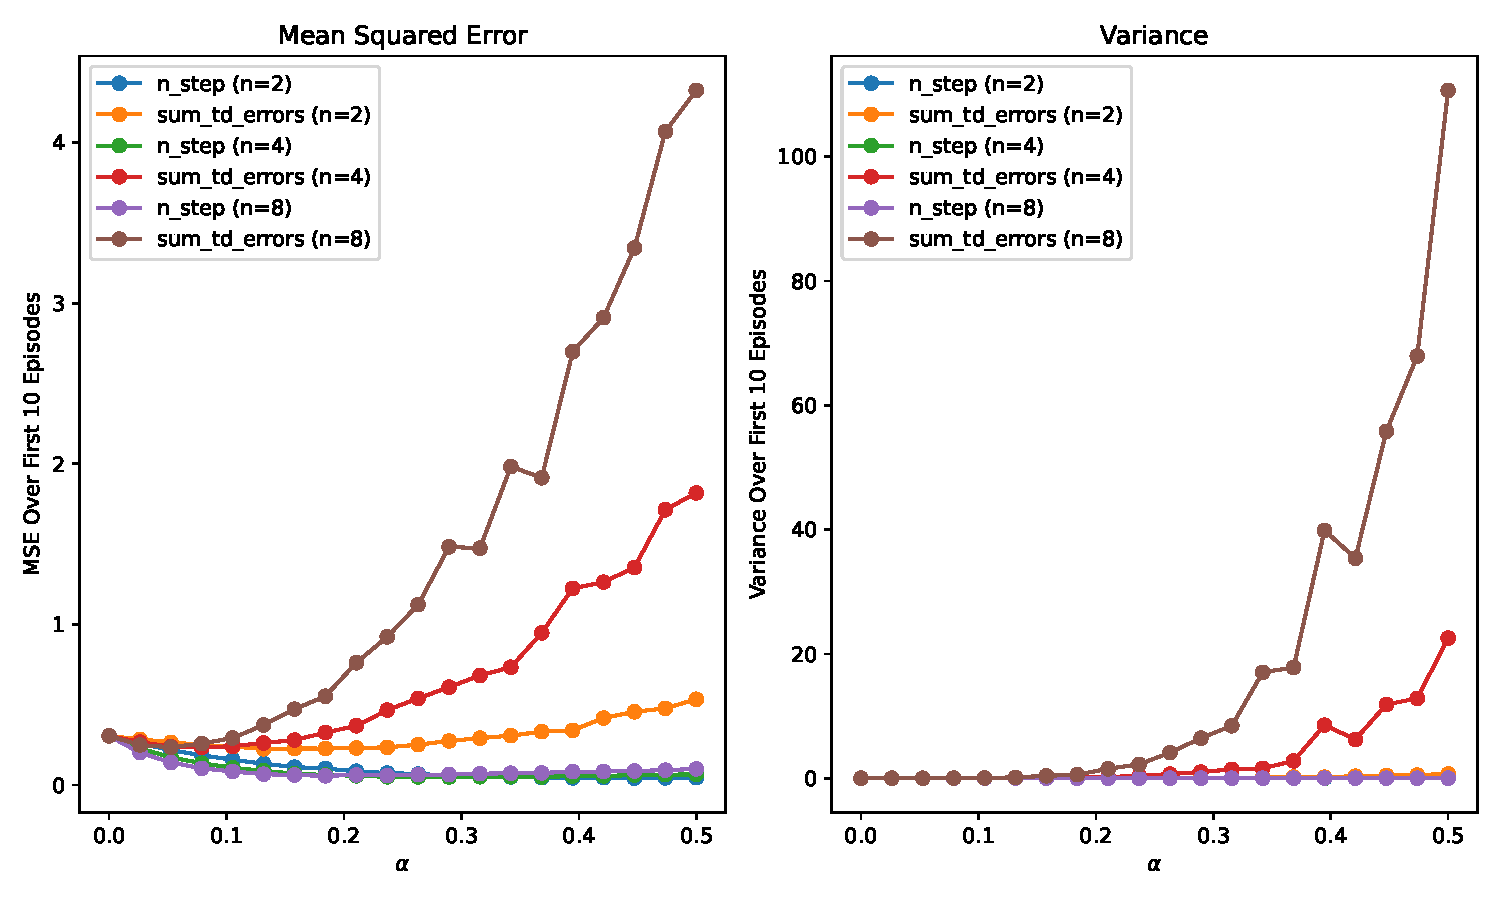
\includegraphics[width=0.8\textwidth]{chapters_latex/figures/ex_07_02.pdf}
    \captionsetup{labelformat=empty}
    \caption{Mean and variance of the MSE after 10 episodes, averaged over 100 runs.}
\end{figure}

\subsection*{Exercise 7.3}
Why do you think a larger random walk task (19 states instead of 5) was
used in the examples of this chapter? Would a smaller walk have shifted the advantage
to a different value of n ? How about the change in left-side outcome from 0 to -1 made
in the larger walk? Do you think that made any difference in the best value of n?

\subsubsection*{Solution:}
The larger task is used to better illustrate the effects of different $n$-step methods due to longer episodes.

With a smaller walk, the advantage would have shifted to a different value of $n$, as the optimal $n$ depends on the length of the episodes.

The change in the left-side outcome from 0 to $-1$ made in the larger walk does not make any difference in the best value of $n$, as the updates are the same, just linearly shifted.

\subsection*{Exercise 7.4}
Prove that the n-step return of Sarsa (7.4) can be written exactly in terms
of a novel TD error, as
\[
G_{t:t+n} = Q_{t-1}(S_t, A_t) + \sum_{k=t}^{\min(t+n, T) - 1} \gamma^{k-t} \left[ R_{k+1} + \gamma Q_k(S_{k+1}, A_{k+1}) - Q_{k-1}(S_k, A_k) \right].
\]

\subsubsection*{Solution:}

\begin{align*}
    G_{t:t+n} &= R_{t+1} \\
    &+ \gamma R_{t+2} \\
    &+ \gamma^2 R_{t+3} \\
    &\cdots \\
    &+ \gamma^{n-1} R_{t+n} \\
    &+ \gamma^n Q_{t+n-1}(S_{t+n}, A_{t+n})  \\
    &= R_{t+1} + Q_{t-1}(S_{t}, A_{t}) - Q_{t-1}(S_{t}, A_{t}) \\
    &+ \gamma R_{t+2} + \gamma  Q_{t}(S_{t+1}, A_{t+1}) -\gamma  Q_{t}(S_{t+1}, A_{t+1})\\
    &+ \gamma^2 R_{t+3} + \gamma^2 Q_{t+1}(S_{t+2}, A_{t+2}) -\gamma^2  Q_{t+1}(S_{t+2}, A_{t+2}) \\
    &\cdots \\
    &+ \gamma^{n-1} R_{t+n} + \gamma^{n-1}Q_{t+n-2}(S_{t+n-1}, A_{t+n-1}) - \gamma^{n-1}Q_{t+n-2}(S_{t+n-1}, A_{t+n-1}) \\
    &+ \gamma^n Q_{t+n-1}(S_{t+n}, A_{t+n}) \\
    &= Q_{t-1}(S_t, A_t) \\
    &+ R_{t+1} + \gamma Q_t(S_{t+1}, A_{t+1}) - Q_{t-1}(S_t, A_t) \\
    &+ \gamma R_{t+2} + \gamma^2 Q_{t+1}(S_{t+2}, A_{t+2}) - \gamma Q_t(S_{t+1}, A_{t+1}) \\
    &+ \gamma^2 R_{t+3} + \gamma^3 Q_{t+2}(S_{t+3}, A_{t+3}) - \gamma^2 Q_{t+1}(S_{t+2}, A_{t+2}) \\
    &\cdots \\
    &+ \gamma^{n-1} R_{t+n} + \gamma^n Q_{t+n-1}(S_{t+n}, A_{t+n}) - \gamma^{n-1} Q_{t+n-2}(S_{t+n-1}, A_{t+n-1}) \\
    &= Q_{t-1}(S_t, A_t) + \sum_{k=t}^{\min(t+n, T) - 1} \gamma^{k-t} \left[ R_{k+1} + \gamma Q_k(S_{k+1}, A_{k+1}) - Q_{k-1}(S_k, A_k) \right].
\end{align*}


\subsection*{Exercise 7.5}
Write the pseudocode for the off-policy state-value prediction algorithm
described above.

\subsubsection*{Solution:}

\fbox{
\begin{minipage}{0.95\textwidth}
\footnotesize
Input: policies $\pi$ and \textcolor{blue}{$b$ (a behavior policy)}

Algorithm parameters: step size $\alpha \in (0,1]$, a positive integer $n$

Initialize $V(s)$ arbitrarily, for all $s \in \mathcal{S}$

All store and access operations (for $S_t$ and $R_t$) can take their index mod $n+1$\\


\textcolor{blue}{
Define function $\bar{G}(t, h)$ as:
\begin{itemize}[left=0em]
    \item[] if $t = h$: return $V(S_h)$
    \item[] if $t = T$: return $0$
    \item[] else: return $\rho_t(R_{t+1} + \gamma \bar{G}(t+1, h)) + (1-\rho_t) V(S_t)$
\end{itemize}
}

Loop for each episode:
\begin{itemize}[left=0em]
    \item[] Initialize and store $S_0 \neq$ terminal
    \item[] $T \leftarrow \infty$
    \item[] Loop for $t = 0, 1, 2, \dots$:
    \begin{itemize}[left=0em]
        \item[] If $t < T$, then:
        \begin{itemize}[left=0em]
            \item[] Take an action according to $b(\cdot | S_t)$
            \item[] \textcolor{blue}{$\rho_t \leftarrow \pi(A_t | S_t) / b(A_t | S_t)$}
            \item[] Observe and store the next reward as $R_{t+1}$ and the next state as $S_{t+1}$
            \item[] If $S_{t+1}$ is terminal, then $T \leftarrow t+1$
        \end{itemize}
        \item[] $\tau \leftarrow t - n + 1$ \hspace{1cm} ($\tau$ is the time whose state's estimate is being updated)
        \item[] If $\tau \geq 0$:
        \begin{itemize}[left=0em]
            \item[] \textcolor{blue}{$G \leftarrow \bar{G}(\tau, \tau+n)$}
            \item[] $V(S_{\tau}) \leftarrow V(S_{\tau}) + \alpha \left[ G - V(S_{\tau}) \right]$
        \end{itemize}
    \end{itemize}
\end{itemize}
Until $\tau = T - 1$

\end{minipage}
}


\subsection*{Exercise 7.6}
Prove that the control variate in the above equations does not change the
expected value of the return.

\subsubsection*{Solution:}
\[
    \mathbb{E}_b \left[ (1 - \rho_t) V_{h-1}(S_t) \right]  = \mathbb{E}_b \left[ (1 - \rho_t) \right] \mathbb{E}_b \left[ V_{h-1}(S_t) \right]  = 0
\]
and

\begin{align*}
    &\mathbb{E}_b \left[ \bar{V}_{h-1}(S_{t+1}) - \rho_{t+1} Q_{h-1}(S_{t+1}, A_{t+1}) \big| S_{t+1} \right] \\
    &= \sum_a \pi(a | S_{t+1}) Q_{h-1}(S_{t+1}, a) - \sum_a b(a | S_{t+1}) \frac{\pi(a | S_{t+1})}{b(a | S_{t+1})} Q_{h-1}(S_{t+1}, a) \\
    &= 0
\end{align*}

\subsection*{*Exercise 7.7}
Write the pseudocode for the off-policy action-value prediction algorithm
described immediately above. Pay particular attention to the termination conditions for
the recursion upon hitting the horizon or the end of episode.

\subsubsection*{Solution:}

\fbox{
\begin{minipage}{0.95\textwidth}
\footnotesize
Input: an arbitrary behavior policy $b$ such that $b(a|s) > 0$, for all $s \in \mathcal{S}, a \in \mathcal{A}$

Initialize $Q(s, a)$ arbitrarily, for all $s \in \mathcal{S}, a \in \mathcal{A}$

Initialize $\pi$ to be greedy with respect to $Q$, or as a fixed given policy

Algorithm parameters: step size $\alpha \in (0, 1]$, a positive integer $n$

All store and access operations (for $S_t$, $A_t$, and $R_t$) can take their index mod $n+1$ \\
\textcolor{blue}{
Define function $\bar{G}(t, h)$ as:
\begin{itemize}[left=0em]
    \item[] if $t = h$: return $Q(S_h, A_h)$
    \item[] if $t = T-1$: return $R_T$
    \item[] else: return \scriptsize{$R_{t+1} + \gamma\rho_{t+1}\left(\bar{G}(t+1, h) -Q(S_{t+1}, A_{t+1}) \right) + \gamma \sum_a \pi(a \mid S_{t+1}) Q(S_{t+1}, a)$}
\end{itemize}
}
Loop for each episode:
\begin{itemize}[left=0em]
    \item[] Initialize and store $S_0 \neq$ terminal
    \item[] Select and store an action $A_0 \sim b(\cdot | S_0)$
    \item[] $T \leftarrow \infty$
    \item[] Loop for $t = 0, 1, 2, \dots$:
    \begin{itemize}[left=0em]
        \item[] If $t < T$, then:
        \begin{itemize}[left=0em]
            \item[] Take action $A_t$
            \item[] Observe and store the next reward as $R_{t+1}$ and the next state as $S_{t+1}$
            \item[] \textcolor{blue}{$\rho_t \leftarrow \pi(A_t | S_t) / b(A_t | S_t)$}
            \item[] If $S_{t+1}$ is terminal, then:
            \begin{itemize}[left=0em]
                \item[] $T \leftarrow t + 1$
            \end{itemize}
            \item[] else:
            \begin{itemize}[left=0em]
                \item[] Select and store an action $A_{t+1} \sim b(\cdot | S_{t+1})$
            \end{itemize}
        \end{itemize}
        \item[] $\tau \leftarrow t - n + 1$ \hspace{1cm} ($\tau$ is the time whose state's estimate is being updated)
        \item[] If $\tau \geq 0$:
        \begin{itemize}[left=0em]
            \item[] \textcolor{blue}{$G \leftarrow \bar{G}(\tau, \tau+n)$}
            \item[] $Q(S_{\tau}, A_{\tau}) \leftarrow Q(S_{\tau}, A_{\tau}) + \alpha \left[ G - Q(S_{\tau}, A_{\tau}) \right]$
            \item[] If $\pi$ is being learned, then ensure that $\pi(\cdot | S_{\tau})$ is greedy with respect to $Q$
        \end{itemize}
    \end{itemize}
\end{itemize}
Until $\tau = T - 1$


\end{minipage}
}


\subsection*{Exercise 7.8}
Show that the general (off-policy) version of the n-step return (7.13) can
still be written exactly and compactly as the sum of state-based TD errors (6.5) if the
approximate state value function does not change.

\subsubsection*{Solution:}
\[
    G_{t:h} = \rho_t(R_{t+1} + \gamma G_{t+1:h}) + (1-\rho_t) V(S_t) = \rho_t(R_{t+1} + \gamma G_{t+1:h} - V(S_t)) + V(S_t)
\]

\begin{align*}
    G_{t:h} - V(S_t) &= \rho_t(R_{t+1} + \gamma G_{t+1:h} - V(S_t)) \\
    &= \rho_t \left(R_{t+1} + \gamma \left[\rho_{t+1}(R_{t+2} + \gamma G_{t+2:h} - V(S_{t+1})) + V(S_{t+1})\right]  - V(S_t) \right) \\
    &= \rho_t \left(R_{t+1} + \gamma V(S_{t+1})  - V(S_t) \right) + \gamma \rho_t \rho_{t+1}(R_{t+2} + \gamma G_{t+2:h} - V(S_{t+1}))\\
    &= \rho_t \delta_t + \gamma \rho_{t:t+1} (R_{t+2} + \gamma G_{t+2:h} - V(S_{t+1})) \\
    &\cdots \\
    &= \sum_{k=t}^{h-1} \gamma^{k-t} \rho_{t:k} \delta_k
\end{align*}


\subsection*{Exercise 7.9}
Repeat the above exercise for the action version of the off-policy n-step
return (7.14) and the Expected Sarsa TD error (the quantity in brackets in Equation 6.9).

\subsubsection*{Solution:}

\[
    G_{t:h} = R_{t+1} + \gamma \rho_{t+1} \left( G_{t+1:h} - Q(S_{t+1}, A_{t+1}) \right) + \gamma \bar{V}(S_{t+1})
\]

where 

\[
    \bar{V}(S_{t+1}) = \sum_a \pi(a | S_{t+1}) Q(S_{t+1}, a).
\]

\[
    \delta_t = R_{t+1} + \gamma \bar{V}(S_{t+1}) - Q(S_t, A_t)
\]

The problem:
\begin{align*}
    G_{t:h} - Q(S_t, A_t) &= R_{t+1} + \gamma \rho_{t+1} \left( G_{t+1:h} - Q(S_{t+1}, A_{t+1}) \right) + \gamma \bar{V}(S_{t+1}) - Q(S_t, A_t) \\
    &= \delta_t + \gamma \rho_{t+1} \left( G_{t+1:h} - Q(S_{t+1}, A_{t+1}) \right) \\
    &= \delta_t + \gamma \rho_{t+1} \left( \delta_{t+1}  + \gamma \rho_{t+2} \left( G_{t+2:h} - Q(S_{t+2}, A_{t+2}) \right) \right) \\
    &= \delta_t + \gamma \rho_{t+1} \delta_{t+1} + \gamma^2 \rho_{t+1:t+2} \left( G_{t+2:h} - Q(S_{t+2}, A_{t+2}) \right) \\
    &\cdots \\
    &= \sum_{k=t}^{h-1} \gamma^{k-t} \rho_{t+1:k} \delta_k
\end{align*}



\subsection*{Exercise 7.10 (programming)}
Devise a small off-policy prediction problem and use it to
show that the off-policy learning algorithm using (7.13) and (7.2) is more data efficient
than the simpler algorithm using (7.1) and (7.9). 

\subsubsection*{Solution:}

See the notebook.

\begin{figure}[H]
    \centering
    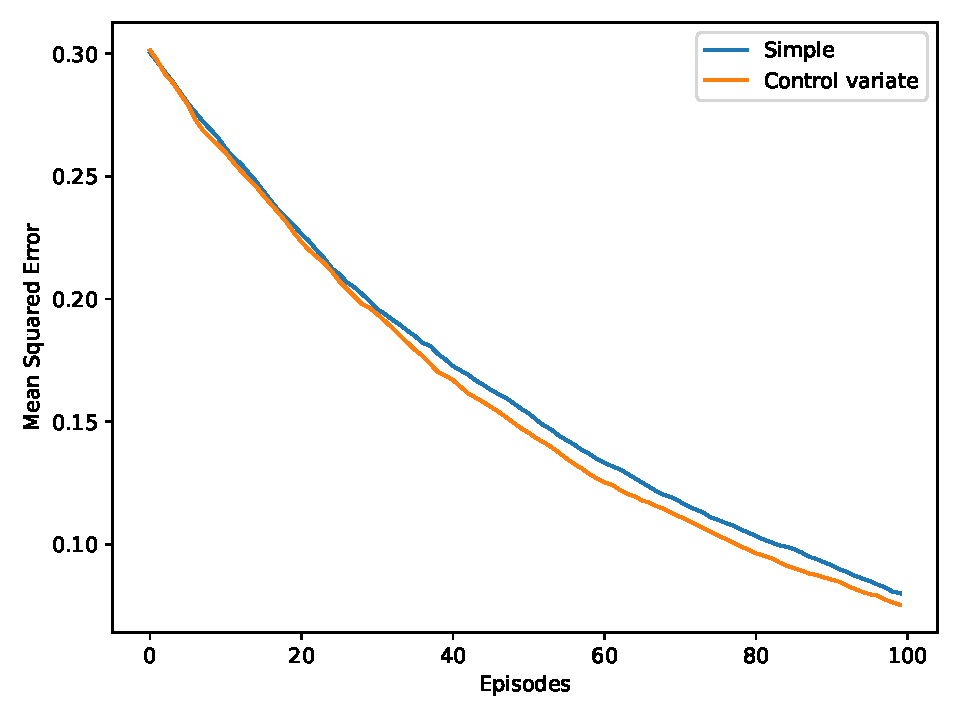
\includegraphics[width=0.8\textwidth]{chapters_latex/figures/ex_07_10.pdf}
    \captionsetup{labelformat=empty}
    \caption{Mean of the MSE after 100 episodes, averaged over 100 runs.}
\end{figure}

\subsection*{Exercise 7.11}
Show that if the approximate action values are unchanging, then the tree-backup return (7.16)
 can be written as a sum of expectation-based TD errors:

\[
G_{t:t+n} = Q(S_t, A_t) + \sum_{k=t}^{\min(t+n-1, T-1)} \delta_k \prod_{i=t+1}^k \gamma \pi(A_i \mid S_i),
\]

where $\delta_t \doteq R_{t+1} + \gamma \bar{V}_t(S_{t+1}) - Q(S_t, A_t)$ and $\bar{V}_t$ is given by (7.8).

\subsubsection*{Solution:}


\begin{align*}
    &G_{t:t+n} = R_{t+1} + \gamma \sum_{a \neq A_{t+1}} \pi(a \mid S_{t+1}) Q_(S_{t+1}, a) 
    + \gamma \pi(A_{t+1} \mid S_{t+1}) G_{t+1:t+n} \\
    &= R_{t+1} + \gamma \bar{V}(S_{t+1}) + \gamma \pi(A_{t+1} \mid S_{t+1}) G_{t+1:t+n} 
    - \gamma \pi(A_{t+1} \mid S_{t+1}) Q(S_{t+1}, A_{t+1}) \\
    &= \delta_t + Q(S_t, A_t)  + \gamma \pi(A_{t+1} \mid S_{t+1}) \left(G_{t+1:t+n} - Q(S_{t+1}, A_{t+1}) \right) \\
    &= \delta_t + Q(S_t, A_t)  + \gamma \pi(A_{t+1} \mid S_{t+1}) \left(\delta_{t+1}  + \gamma \pi(A_{t+2} \mid S_{t+2}) \left(G_{t+2:t+n} - Q(S_{t+2}, A_{t+2}) \right) \right)\\
    &\cdots \\
    &= Q(S_t, A_t) + \sum_{k=t}^{\min(t+n-1, T-1)} \delta_k \prod_{i=t+1}^k \gamma \pi(A_i \mid S_i)
\end{align*}
%\begin{align*}
%    G_{t:t+n} &= R_{t+1} + \gamma \bar{V}_t(S_{t+1}) \\
%    &+ \gamma \pi(A_{t+1} | S_{t+1}) \left[ R_{t+2} + \gamma \bar{V}_t(S_{t+2}) \right] \\
%    &+ \gamma \pi(A_{t+1} | S_{t+1}) \gamma \pi(A_{t+2} | S_{t+2}) \left[ R_{t+3} + \gamma \bar{V}_t(S_{t+3}) \right] \\
%    &\cdots \\
%    &+ \gamma \pi(A_{t+1} | S_{t+1}) \gamma \pi(A_{t+2} | S_{t+2}) \cdots \gamma \pi(A_{t+n-1} | S_{t+n-1}) \left[ R_{t+n} + \gamma \bar{V}_t(S_{t+n}) \right] \\
%    &= Q(S_t, A_t) + \sum_{k=t}^{\min(t+n-1, T-1)} \delta_k \prod_{i=t+1}^k \gamma \pi(A_i \mid S_i)
%\end{align*}
\section*{Chapter 8}

\subsection*{Exercise 8.1}
The nonplanning method looks particularly poor in Figure 8.3 because it is
a one-step method; a method using multi-step bootstrapping would do better. Do you
think one of the multi-step bootstrapping methods from Chapter 7 could do as well as
the Dyna method? Explain why or why not.

\subsection*{Solution}
While multi-step bootstrapping methods can improve over one-step methods and perform
reasonably well, they are unlikely to match the performance of the Dyna method. The key
difference lies in the use of a model: Dyna exploits the additional simulated experience
generated by the model to accelerate learning, something that multi-step methods cannot
achieve.

\subsection*{Exercise 8.2}
Why did the Dyna agent with exploration bonus, Dyna-Q+, perform
better in the first phase as well as in the second phase of the blocking and shortcut
experiments?

\subsection*{Solution}

In Phase 1, the Dyna-Q+ agent performed better because its exploration bonus encouraged
it to visit less-explored state-action pairs. The Dyna-Q agent did not have this,
so it was trying to search for the optimal path randomly.

\subsection*{Exercise 8.3}
Careful inspection of Figure 8.5 reveals that the difference between Dyna-Q+
and Dyna-Q narrowed slightly over the first part of the experiment. What is the reason
for this?

\subsection*{Solution}
The exploration term in Dyna-Q+ is bigger than the exploration term in Dyna-Q, so it takes
suboptimal actions more often, consequently bringing the slope of the cumulative reward down.

\subsection*{Exercise 8.4 (programming)}
The exploration bonus described above actually changes
the estimated values of states and actions. Is this necessary? Suppose the bonus $\kappa \sqrt{\tau}$
was used not in updates, but solely in action selection. That is, suppose the action
selected was always that for which $Q(S t, a) + \kappa \sqrt{\tau(S_t, a)}$ was maximal. Carry out a
gridworld experiment that tests and illustrates the strengths and weaknesses of this
alternate approach. 

\subsection*{Solution}
See the notebook.

\begin{figure}[H]
    \centering
    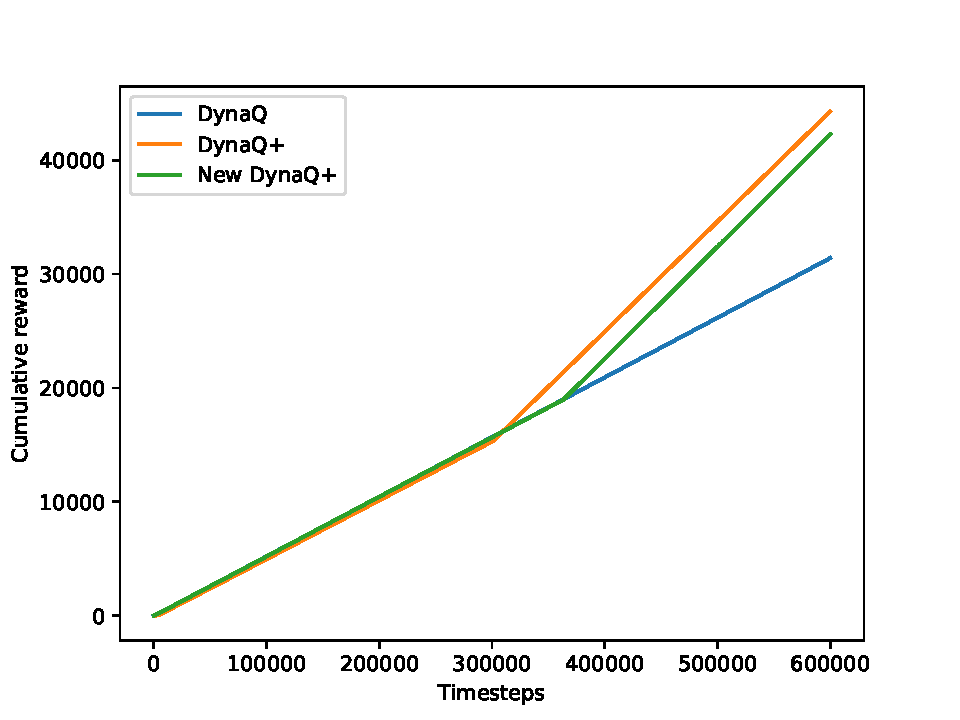
\includegraphics[width=0.8\textwidth]{chapters_latex/figures/ex_08_04.pdf}
    \captionsetup{labelformat=empty}
\end{figure}

There seems to be no significant difference between the two methods, in this case, but this may be just a coincidence. If the agent is at the shorcut location, and doesn't choose the \textit{up} action, then we have to wait again for the agent to go there again, which may take a lot of time.

\subsection*{Exercise 8.5}
How might the tabular Dyna-Q algorithm shown on page 164 be modified
to handle stochastic environments? How might this modification perform poorly on
changing environments such as considered in this section? How could the algorithm be
modified to handle stochastic environments $\textit{and}$ changing environments? 

\subsection*{Solution}

We could save all the \textit{next state} and \textit{reward} pairs, and then sample from them when updating the Q-values. This would perform poorly on changing environments because the agent would be updating its Q-values with outdated information.

To handle both stochastic and changing environments, we could give more weight to the most recent experiences, and less weight to the older ones. This way, the agent would be able to adapt to the changes in the environment, and even forget about the old experiences if they are not relevant anymore.

\subsection*{Exercise 8.6}
The analysis above assumed that all of the \textit{b} possible next states were
equally likely to occur. Suppose instead that the distribution was highly skewed, that
some of the b states were much more likely to occur than most. Would this strengthen or
weaken the case for sample updates over expected updates? Support your answer. 

\subsection*{Solution}
A skewed distribution strengthens the case for sample updates because they naturally focus on the most likely transitions, improving computational efficiency. However, if rare transitions are important, expected updates are better as they account for all possible outcomes. Thus, the preference depends on the importance of rare events in the problem.

\subsection*{Exercise 8.7}
Some of the graphs in Figure 8.8 seem to be scalloped in their early portions,
particularly the upper graph for $b = 1$ and the uniform distribution. Why do you think
this is? What aspects of the data shown support your hypothesis? 

\subsection*{Solution}

The scalloped pattern arises because, for $b=1$ and the uniform distribution, value estimates improve significantly when new states are encountered for the first time. This creates periodic jumps in learning, as updates depend entirely on the order of state visits. Over time, as all states are visited and value estimates stabilize, the pattern smooths out.

\subsection*{Exercise 8.8 (programming)}
Replicate the experiment whose results are shown in the
lower part of Figure 8.8, then try the same experiment but with b = 3. Discuss the
meaning of your results.

\subsection*{Solution}
See the notebook.

\begin{figure}[H]
    \centering
    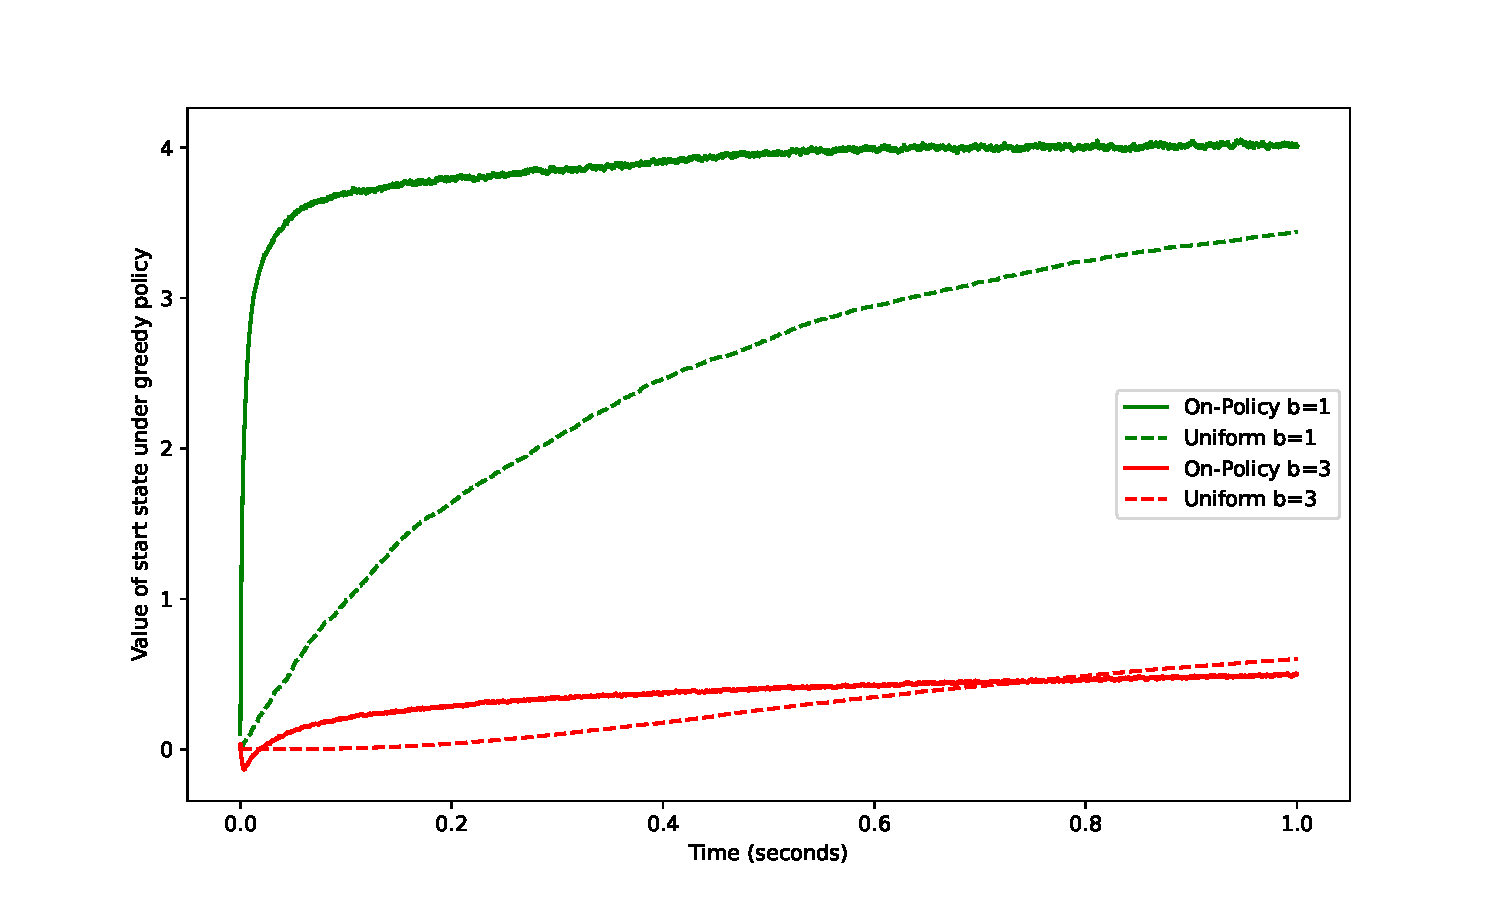
\includegraphics[width=0.9\textwidth]{chapters_latex/figures/ex_08_08.pdf}
    \captionsetup{labelformat=empty}
\end{figure}

The results discussed in the book can be seen: "The effect was stronger, and the initial period of faster planning was longer, at smaller branching factors. In other experiments, we found that these effects also became stronger as the number of states increased".
\section*{Chapter 9}

\subsection*{Exercise 9.1}

Show that tabular methods such as presented in Part I of this book are a special case of linear function approximation. What would the feature vectors be?

\subsection*{Solution}

Tabular methods are a special case of linear function approximation where each state is represented by a one-hot feature vector $\mathbf{x}(s)$. For a state $s_i$ in a space of $n$ states, $\mathbf{x}(s_i)$ is an $n$-dimensional vector with a $1$ at the $i$-th position and $0$ elsewhere. The value function is then:

\[
\hat{v}(s, \mathbf{w}) = \mathbf{x}(s)^\top \mathbf{w},
\]

where $\mathbf{w}$ is the vector of state values.

The SGD update rule then becomes:

\begin{align*}
    \mathbf{w}_{t+1} &= \mathbf{w}_t + \alpha \left[ U_t - \hat{v}(S_t, \mathbf{w}_t) \right] \nabla \hat{v}(S_t, \mathbf{w}_t) \\
    &= \mathbf{w}_t + \alpha \left[ U_t - \mathbf{x}(S_t)^\top \mathbf{w}_t \right] \mathbf{x}(S_t) \\
    &= \mathbf{w}_t + \alpha \left[ U_t - \mathbf{w}_t^{(S_t)}  \right] e_{S_t} \\
\end{align*}

Which is analogous to the tabular update rule:
\[
V_{t+1}(S_t) = V_t(S_t) + \alpha \left[ U_t - V_t(S_t) \right]
\]



\subsection*{Exercise 9.2}

Why does (9.17) define $(n + 1)^k$ distinct features for dimension $k$?

\subsection*{Solution}

Each of the $k$ dimensions independently contributes $(n+1)$ choices for the degree of the polynomial, so the total unique combinations of features is $(n+1)^k$.

\subsection*{Exercise 9.3}

What $n$ and $c_{i,j}$ produce the feature vectors $\mathbf{x}(s) = (1, s_1, s_2, s_1s_2, s_1^2, s_2^2, s_1s_2^2, s_1^2 s_2, s_1^2 s_2^2)^\top$?

\subsection*{Solution}

There are 2 states, and the maximum degree of the features is 2, so both $n$ and $k$ are 2. The coefficients $c_{i,j}$ are:
\[
C = \begin{bmatrix}
    0 & 0 \\
    1 & 0 \\
    0 & 1 \\
    1 & 1 \\
    2 & 0 \\
    0 & 2 \\
    1 & 2 \\
    2 & 1 \\
    2 & 2 \\
\end{bmatrix}
\]

\subsection*{Exercise 9.4}

Suppose we believe that one of two state dimensions is more likely to have
an effect on the value function than is the other, that generalization should be primarily
across this dimension rather than along it. What kind of tilings could be used to take
advantage of this prior knowledge?

\subsection*{Solution}

We need to use a tiling that is similar to the Asymmetric generalization in Figure 9.7. The tiling should have more tiles along the dimension that is more likely to have an effect on the value function.

\subsection*{Exercise 9.5}
Suppose you are using tile coding to transform a seven-dimensional continuous
state space into binary feature vectors to estimate a state value function $\hat{v}(s, \mathbf{w}) \approx v_\pi(s)$.
You believe that the dimensions do not interact strongly, so you decide to use eight tilings
of each dimension separately (stripe tilings), for $7 \times 8 = 56$ tilings. In addition, in case
there are some pairwise interactions between the dimensions, you also take all  ${{7}\choose{2}} = 21$
pairs of dimensions and tile each pair conjunctively with rectangular tiles. You make
two tilings for each pair of dimensions, making a grand total of $21 \times 2 + 56 = 98$ tilings.
Given these feature vectors, you suspect that you still have to average out some noise,
so you decide that you want learning to be gradual, taking about 10 presentations with
the same feature vector before learning nears its asymptote. What step-size parameter $\alpha$
should you use? Why?

\subsection*{Solution}
The feature vectors always have 98 1s, because each tiling only has exactly one tile activated, so $\mathbf{x}^\top \mathbf{x}$ is always 98. Thus $\alpha = \left(\tau \times \mathbb{E}[\mathbf{x}^\top \mathbf{x}]\right)^{-1} = \frac{1}{10 \times 98} = \frac{1}{980}$.

\subsection*{Exercise 9.6}
If $\tau = 1$ and $\mathbf{x}(S_t)^\top \mathbf{x}(S_t) = \mathbb{E}[\mathbf{x}^\top \mathbf{x}]$, prove that (9.19) together with (9.7)
and linear function approximation results in the error being reduced to zero in one update.

\subsection*{Solution}
Based on (9.19):
\[
    \alpha = \left( \tau \times \mathbb{E}[\mathbf{x}^\top \mathbf{x}] \right)^{-1} = \left( 1 \times \mathbf{x}(S_t)^\top \mathbf{x}(S_t) \right)^{-1} = \frac{1}{\mathbf{x}(S_t)^\top \mathbf{x}(S_t)}
\]

The update rule (9.7) for linear function approximation: 
\[
    \mathbf{w}_{t+1} = \mathbf{w}_t + \alpha \left[ U_t - \mathbf{x}(S_t)^\top \mathbf{w}_t \right] \mathbf{x}(S_t)
\]

The output for the new weight:
\begin{align*}
    \mathbf{w}_{t+1}^\top \mathbf{x}(S_t) &= \mathbf{w}_t^\top \mathbf{x}(S_t) + \alpha \left[ U_t - \mathbf{x}(S_t)^\top \mathbf{w}_t \right] \mathbf{x}(S_t)^\top \mathbf{x}(S_t) \\
    &= \mathbf{w}_t^\top \mathbf{x}(S_t) + \frac{1}{\mathbf{x}(S_t)^\top \mathbf{x}(S_t)} \left[ U_t - \mathbf{x}(S_t)^\top \mathbf{w}_t \right] \mathbf{x}(S_t)^\top \mathbf{x}(S_t)  \\
    &= \mathbf{w}_t^\top \mathbf{x}(S_t) + U_t - \mathbf{x}(S_t)^\top \mathbf{w}_t \\
    &= U_t
\end{align*}


\subsection*{Exercise 9.7}

One of the simplest artificial neural networks consists of a single semi-linear
unit with a logistic nonlinearity. The need to handle approximate value functions of this
form is common in games that end with either a win or a loss, in which case the value of
a state can be interpreted as the probability of winning. Derive the learning algorithm
for this case, from (9.7), such that no gradient notation appears.

\subsection*{Solution}


The logistic function is defined as:
\[
    \sigma(x) = \frac{1}{1 + e^{-x}}
\]

The derivative of the logistic function is:
\[
    \sigma'(x) = \sigma(x) (1 - \sigma(x))
\]

Using this, we can derive the learning algorithm for a single semi-linear unit with a logistic nonlinearity. The value function is:
\[
    \hat{v}(s, \mathbf{w}) = \sigma(\mathbf{x}(s)^\top \mathbf{w})
\]

The update rule (9.7) for linear function approximation is:
\[
    \mathbf{w}_{t+1} = \mathbf{w}_t + \alpha \left[ U_t - \hat{v}(S_t, \mathbf{w}_t) \right] \nabla \hat{v}(S_t, \mathbf{w}_t)
\]

Substituting the logistic function and its derivative:
\[
    \nabla \hat{v}(S_t, \mathbf{w}_t) = \sigma'(\mathbf{x}(S_t)^\top \mathbf{w}_t) \mathbf{x}(S_t) = \sigma(\mathbf{x}(S_t)^\top \mathbf{w}_t) (1 - \sigma(\mathbf{x}(S_t)^\top \mathbf{w}_t)) \mathbf{x}(S_t)
\]

Thus, the update rule becomes:
\[
    \mathbf{w}_{t+1} = \mathbf{w}_t + \alpha \left[ U_t - \sigma(\mathbf{x}(S_t)^\top \mathbf{w}_t) \right] \sigma(\mathbf{x}(S_t)^\top \mathbf{w}_t) (1 - \sigma(\mathbf{x}(S_t)^\top \mathbf{w}_t)) \mathbf{x}(S_t)
\]

Substituting $\hat{v}$, we get:
\[
    \mathbf{w}_{t+1} = \mathbf{w}_t + \alpha \left[ U_t - \hat{v}(S_t, \mathbf{w}_t) \right] \hat{v}(S_t, \mathbf{w}_t) (1 - \hat{v}(S_t, \mathbf{w}_t)) \mathbf{x}(S_t)
\]


\subsection*{*Exercise 9.8}
Arguably, the squared error used to derive (9.7) is inappropriate for the
case treated in the preceding exercise, and the right error measure is the \textit{cross-entropy
loss} (which you can find on Wikipedia). Repeat the derivation in Section 9.3, using the
cross-entropy loss instead of the squared error in (9.4), all the way to an explicit form
with no gradient or logarithm notation in it. Is your final form more complex, or simpler,
than that you obtained in the preceding exercise?

\subsection*{Solution}

The cross-entropy loss for a binary classification problem is defined as:
\[ 
    L(U_t, \hat{v}(S_t, \mathbf{w})) = - U_t \log(\hat{v}(S_t, \mathbf{w})) - (1 - U_t) \log(1 - \hat{v}(S_t, \mathbf{w}))
\]

The gradient of the cross-entropy loss with respect to the weights is:
\[ 
    \nabla L(U_t, \hat{v}(S_t, \mathbf{w})) = - \frac{U_t}{\hat{v}(S_t, \mathbf{w})} \nabla \hat{v}(S_t, \mathbf{w}) + \frac{1 - U_t}{1 - \hat{v}(S_t, \mathbf{w})} \nabla \hat{v}(S_t, \mathbf{w})
\]

Using the logistic function and its derivative:
\[ 
    \nabla \hat{v}(S_t, \mathbf{w}) = \hat{v}(S_t, \mathbf{w}) (1 - \hat{v}(S_t, \mathbf{w})) \mathbf{x}(S_t)
\]

Substituting this into the gradient of the cross-entropy loss:
\begin{align*} 
    \nabla L(U_t, \hat{v}(S_t, \mathbf{w})) = &- \frac{U_t}{\hat{v}(S_t, \mathbf{w})} \hat{v}(S_t, \mathbf{w}) (1 - \hat{v}(S_t, \mathbf{w})) \mathbf{x}(S_t) \\
    &+ \frac{1 - U_t}{1 - \hat{v}(S_t, \mathbf{w})} \hat{v}(S_t, \mathbf{w}) (1 - \hat{v}(S_t, \mathbf{w})) \mathbf{x}(S_t)
\end{align*}

Simplifying:
\[ 
    \nabla L(U_t, \hat{v}(S_t, \mathbf{w})) = - U_t (1 - \hat{v}(S_t, \mathbf{w})) \mathbf{x}(S_t) + (1 - U_t) \hat{v}(S_t, \mathbf{w}) \mathbf{x}(S_t)
\]
\[ 
    \nabla L(U_t, \hat{v}(S_t, \mathbf{w})) = (\hat{v}(S_t, \mathbf{w}) - U_t) \mathbf{x}(S_t)
\]

The update rule for the weights using the cross-entropy loss is:
\begin{align*}
    \mathbf{w}_{t+1} &= \mathbf{w}_t - \alpha \nabla L(U_t, \hat{v}(S_t, \mathbf{w}_t)) \\
    \mathbf{w}_{t+1} &= \mathbf{w}_t - \alpha (\hat{v}(S_t, \mathbf{w}_t) - U_t) \mathbf{x}(S_t)
\end{align*}

Thus, the final update rule is:
\[ 
    \mathbf{w}_{t+1} = \mathbf{w}_t + \alpha (U_t - \hat{v}(S_t, \mathbf{w}_t)) \mathbf{x}(S_t)
\]

This form is simpler than the one obtained in the preceding exercise.
\section*{Chapter 10}

\subsection*{Exercise 10.1}

We have not explicitly considered or given pseudocode for any Monte Carlo
methods in this chapter. What would they be like? Why is it reasonable not to give
pseudocode for them? How would they perform on the Mountain Car task?
\subsubsection*{Solution:}

Monte Carlo methods are basically n-step methods with $n$ equal to the length of the episode  ($T$).
The pseudocode doesn't need many changes from the n-step methods, the only difference is that $n$ is always equal to $T$.

Based on Figure 10.4, we can see that the agent behaves worse with the increase of $n$, so Monte Carlo methods would perform poorly on the task.

\subsection*{Exercise 10.2}

Give pseudocode for semi-gradient one-step Expected Sarsa for control.

\subsubsection*{Solution:}

\fbox{
\begin{minipage}{0.95\textwidth}
\footnotesize 
    Input: a differentiable action-value function parameterization $\hat{q} : \mathcal{S} \times \mathcal{A} \times \mathbb{R}^d \to \mathbb{R}$

    Algorithm parameters: step size $\alpha > 0$, small $\epsilon > 0$

    Initialize value-function weights $\mathbf{w} \in \mathbb{R}^d$ arbitrarily (e.g., $\mathbf{w} = \mathbf{0}$)


    Loop for each episode:
    \begin{itemize}[left=0em]
        \item[] $S, A \leftarrow$ initial state and action of episode (e.g., $\epsilon$-greedy)
        \item[] Loop for each step of episode:
        \begin{itemize}[left=0em]
            \item[] Take action $A$, observe $R, S'$
            \item[] If $S'$ is terminal:
            \begin{itemize}[left=0em]
                \item[] $\mathbf{w} \leftarrow \mathbf{w} + \alpha \left[ R - \hat{q}(S, A, \mathbf{w}) \right] \nabla \hat{q}(S, A, \mathbf{w})$
                \item[] Go to next episode
            \end{itemize}
            \item[] Choose $A'$ as a function of $\hat{q}(S', \cdot, \mathbf{w})$ (e.g., $\epsilon$-greedy)
            \item[] \textcolor{blue}{$\mathbf{w} \leftarrow \mathbf{w} + \alpha \left[ R + \gamma \sum_a \pi(a | S') \hat{q}(S', a, \mathbf{w}) - \hat{q}(S, A, \mathbf{w}) \right] \nabla \hat{q}(S, A, \mathbf{w})$}
            \item[] $S \leftarrow S'$
            \item[] $A \leftarrow A'$
        \end{itemize}
    \end{itemize}
\end{minipage}
}


\subsection*{Exercise 10.3}

Why do the results shown in Figure 10.4 have higher standard errors at
large $n$ than at small $n$?

\subsubsection*{Solution:}

The higher standard errors at large $n$ arise due to the accumulation of errors over multiple steps (with regard to action selection) and delayed updates. 

\subsection*{Exercise 10.4}

Give pseudocode for a differential version of semi-gradient Q-learning.

\subsubsection*{Solution:}

\fbox{
\begin{minipage}{0.95\textwidth}
\footnotesize 
    Input: a differentiable action-value function parameterization $\hat{q} : \mathcal{S} \times \mathcal{A} \times \mathbb{R}^d \to \mathbb{R}$

    Algorithm parameters: step sizes $\alpha, \beta > 0$, small $\epsilon > 0$

    Initialize value-function weights $\mathbf{w} \in \mathbb{R}^d$ arbitrarily (e.g., $\mathbf{w} = \mathbf{0}$)

    Initialize average reward estimate $\bar{R} \in \mathbb{R}$ arbitrarily (e.g., $\bar{R} = 0$)
    

    \textcolor{blue}{Initialize state $S$}

    Loop for each step:
    \begin{itemize}[left=0em]
        \item[] \textcolor{blue}{Choose $A$ as a function of $\hat{q}(S, \cdot, \mathbf{w})$ (e.g., $\epsilon$-greedy)}
        \item[] Take action $A$, observe $R, S'$
        \item[] \textcolor{blue}{$A' \leftarrow \argmax_{a'} \hat{q}(S', a', \mathbf{w})$}
        \item[] $\delta \leftarrow R - \bar{R} + \hat{q}(S', A', \mathbf{w}) - \hat{q}(S, A, \mathbf{w})$
        \item[] $\bar{R} \leftarrow \bar{R} + \beta \delta$
        \item[] $\mathbf{w} \leftarrow \mathbf{w} + \alpha \delta \nabla \hat{q}(S, A, \mathbf{w})$
        \item[] $S \leftarrow S'$
    \end{itemize}
\end{minipage}
}

\subsection*{Exercise 10.5}
What equations are needed (beyond 10.10) to specify the differential version of TD(0)?

\subsubsection*{Solution:}

\[
    \mathbf{w}_{t+1} = \mathbf{w}_t + \alpha \delta_t \nabla \hat{v}(S_t, \mathbf{w}_t)
\]

\subsection*{Exercise 10.6}

Suppose there is an MDP that under any policy produces the deterministic
sequence of rewards $+1$, $0$, $+1$, $0$, $+1$, $0$, $\dots$ going on forever. Technically, this violates
ergodicity; there is no stationary limiting distribution $\mu_\pi$ and the limit (10.7) does not
exist. Nevertheless, the average reward (10.6) is well defined. What is it? Now consider
two states in this MDP. From $\mathsf{A}$, the reward sequence is exactly as described above,
starting with a $+1$, whereas, from $\mathsf{B}$, the reward sequence starts with a $0$ and then
continues with $+1$, $0$, $+1$, $0$, $\dots$. We would like to compute the differential values of $\mathsf{A}$ and
$\mathsf{B}$. Unfortunately, the differential return (10.9) is not well defined when starting from
these states as the implicit limit does not exist. To repair this, one could alternatively
define the differential value of a state as
\[
    v_\pi(s) \doteq \lim_{\gamma \rightarrow 1} \lim_{h \rightarrow \infty} \sum_{t=0}^{h} \gamma^t \left( \mathbb{E} \left[ R_{t+1} \mid S_0 = s \right] - r(\pi) \right).
\]
Under this definition, what are the differential values of states $\mathsf{A}$ and $\mathsf{B}$?

\subsubsection*{Solution:}
\[
    \lim_{h \rightarrow \infty} \frac{1}{h} \sum_{t=1}^{h} \mathbb{E} \left[ R_{t} \mid S_0, A_{0:t-1} \sim  \pi \right] = \lim_{h \rightarrow \infty} \frac{1}{h}  \left\lfloor \frac{h+1}{2} \right\rfloor = \frac{1}{2}
\]

Differential value of state $\mathsf{A}$:
\begin{align*}
    \lim_{\gamma \rightarrow 1} \lim_{h \rightarrow \infty} \sum_{t=0}^{h} \gamma^t \left( \mathbb{E} \left[ R_{t+1} \mid S_0 = \mathsf{A} \right] - r(\pi) \right) &=  \lim_{\gamma \rightarrow 1} \lim_{h \rightarrow \infty} \sum_{t=0}^{h} \frac{1}{2}\left(-\gamma\right)^t \\
    &= \frac{1}{2}\lim_{\gamma \rightarrow 1} \frac{1}{1 + \gamma} \\
    &= \frac{1}{4}
\end{align*}

Differential value of state $\mathsf{B}$:
\begin{align*}
    \lim_{\gamma \rightarrow 1} \lim_{h \rightarrow \infty} \sum_{t=0}^{h} \gamma^t \left( \mathbb{E} \left[ R_{t+1} \mid S_0 = \mathsf{B} \right] - r(\pi) \right) &=  \lim_{\gamma \rightarrow 1} \lim_{h \rightarrow \infty} \sum_{t=0}^{h} -\frac{1}{2}\left(-\gamma\right)^t \\
    &= -\frac{1}{2}\lim_{\gamma \rightarrow 1} \frac{1}{1 + \gamma} \\
    &= -\frac{1}{4}
\end{align*}

\subsection*{Exercise 10.7}

Consider a Markov reward process consisting of a ring of three states $\mathsf{A}$, $\mathsf{B}$,
and $\mathsf{C}$, with state transitions going deterministically around the ring. A reward of +1 is
received upon arrival in $\mathsf{A}$ and otherwise the reward is 0. What are the differential values
of the three states, using (10.13)? 

\subsubsection*{Solution:}
The average reward is $r(\pi)=\frac{1}{3}$.

Differential value of state $\mathsf{A}$:
\begin{align*}
    \lim_{\gamma \rightarrow 1} \lim_{h \rightarrow \infty} \sum_{t=0}^{h} \gamma^t \left( \mathbb{E} \left[ R_{t+1} \mid S_0 = \mathsf{A} \right] - r(\pi) \right) &=  \lim_{\gamma \rightarrow 1} \lim_{h \rightarrow \infty} \sum_{t=0}^{h} -\frac{1}{3} \gamma^{3t} -\frac{1}{3} \gamma^{3t+1}  + \frac{2}{3} \gamma^{3t+2} \\
    &= \lim_{\gamma \rightarrow 1} \lim_{h \rightarrow \infty} \sum_{t=0}^{h} (\gamma^3)^t \frac{2\gamma^2 - \gamma - 1}{3} \\
    &= \lim_{\gamma \rightarrow 1} \frac{2\gamma^2 - \gamma - 1}{3 - 3\gamma^3} \\
    &= \lim_{\gamma \rightarrow 1} \frac{4\gamma - 1}{-9\gamma^2} \\
    &= - \frac{1}{3}
\end{align*}

Differential value of state $\mathsf{B}$:
\begin{align*}
    \lim_{\gamma \rightarrow 1} \lim_{h \rightarrow \infty} \sum_{t=0}^{h} \gamma^t \left( \mathbb{E} \left[ R_{t+1} \mid S_0 = \mathsf{B} \right] - r(\pi) \right) &=  \lim_{\gamma \rightarrow 1} \lim_{h \rightarrow \infty} \sum_{t=0}^{h} -\frac{1}{3} \gamma^{3t} +\frac{2}{3} \gamma^{3t+1}  - \frac{1}{3} \gamma^{3t+2} \\
    &= \lim_{\gamma \rightarrow 1} \lim_{h \rightarrow \infty} \sum_{t=0}^{h} (\gamma^3)^t \frac{-\gamma^2 + 2\gamma - 1}{3} \\
    &= \lim_{\gamma \rightarrow 1} \frac{-\gamma^2 + 2\gamma - 1}{3 - 3\gamma^3} \\
    &= \lim_{\gamma \rightarrow 1} \frac{-2\gamma + 2}{-9\gamma^2} \\
    &= 0
\end{align*}

Differential value of state $\mathsf{C}$:
\begin{align*}
    \lim_{\gamma \rightarrow 1} \lim_{h \rightarrow \infty} \sum_{t=0}^{h} \gamma^t \left( \mathbb{E} \left[ R_{t+1} \mid S_0 = \mathsf{C} \right] - r(\pi) \right) &=  \lim_{\gamma \rightarrow 1} \lim_{h \rightarrow \infty} \sum_{t=0}^{h} \frac{2}{3} \gamma^{3t} -\frac{1}{3} \gamma^{3t+1}  - \frac{1}{3} \gamma^{3t+2} \\
    &= \lim_{\gamma \rightarrow 1} \lim_{h \rightarrow \infty} \sum_{t=0}^{h} (\gamma^3)^t \frac{-\gamma^2 - \gamma + 2}{3} \\
    &= \lim_{\gamma \rightarrow 1} \frac{-\gamma^2 -\gamma + 2}{3 - 3\gamma^3} \\
    &= \lim_{\gamma \rightarrow 1} \frac{-2\gamma - 1}{-9\gamma^2} \\
    &= \frac{1}{3}
\end{align*}

\subsection*{Exercise 10.8}

The pseudocode in the box on page 251 updates $\bar{R}_t$ using  $\delta_t$ as an error
rather than simply $R_{t+1} - \bar{R}_t$. Both errors work, but using $\delta_t$ is better. To see why,
consider the ring MRP of three states from Exercise 10.7. The estimate of the average
reward should tend towards its true value of $\frac{1}{3}$. Suppose it was already there and was
held stuck there. What would the sequence of $R_{t+1} - \bar{R}_t$ errors be? What would the
sequence of $\delta_t$ errors be (using Equation 10.10)? Which error sequence would produce
a more stable estimate of the average reward if the estimate were allowed to change in
response to the errors? Why?

\subsubsection*{Solution:}

Sequence of $R_{t+1} - \bar{R}_t$ errors (starting from $\mathsf{A}$):

\[
    - \frac{1}{3}, - \frac{1}{3}, \frac{2}{3}, - \frac{1}{3}, - \frac{1}{3}, \frac{2}{3}, \dots
\]

Sequence of $\delta_t$ errors (starting from $\mathsf{A}$):
\[
    - \frac{1}{3} + 0 + \frac{1}{3}, - \frac{1}{3} + \frac{1}{3} - 0, \frac{2}{3} - \frac{1}{3} - \frac{1}{3}, \dots = 0,0,0,0,0,0, \dots
\]

The sequence of $\delta_t$ errors would produce a more stable estimate of the average reward, as it would always be zero.

\subsection*{Exercise 10.9}

In the differential semi-gradient $n$-step Sarsa algorithm, the step-size
parameter on the average reward, $\beta$, needs to be quite small so that $\bar{R}$ becomes a good
long-term estimate of the average reward. Unfortunately, $\bar{R}$ will then be biased by its
initial value for many steps, which may make learning inefficient. Alternatively, one could
use a sample average of the observed rewards for $\bar{R}$. That would initially adapt rapidly
but in the long run would also adapt slowly. As the policy slowly changed, $\bar{R}$ would also
change; the potential for such long-term nonstationarity makes sample-average methods
ill-suited. In fact, the step-size parameter on the average reward is a perfect place to use
the unbiased constant-step-size trick from Exercise 2.7. Describe the specific changes
needed to the boxed algorithm for differential semi-gradient $n$-step Sarsa to use this
trick.

\subsubsection*{Solution:}
\fbox{
\begin{minipage}{0.95\textwidth}
    \footnotesize 

    Input: a differentiable function $\hat{q} : \mathcal{S} \times \mathcal{A} \times \mathbb{R}^d \to \mathbb{R}$, a policy $\pi$

    Initialize value-function weights $\mathbf{w} \in \mathbb{R}^d$ arbitrarily (e.g., $\mathbf{w} = \mathbf{0}$)

    Initialize average-reward estimate $\bar{R} \in \mathbb{R}$ arbitrarily (e.g., $\bar{R} = 0$)

    Algorithm parameters: step sizes $\alpha, \beta > 0$, small $\epsilon > 0$, a positive integer $n$

    All store and access operations ($S_t$, $A_t$, and $R_t$) can take their index mod $n+1$

    Initialize and store $S_0$ and $A_0$

    \textcolor{blue}{$\bar{o} \leftarrow 0$}

    Loop for each step, $t = 0, 1, 2, \dots$:
    \begin{itemize}[left=0em]
        \item[] Take action $A_t$
        \item[] Observe and store the next reward as $R_{t+1}$ and the next state as $S_{t+1}$
        \item[] Select and store an action $A_{t+1} \sim \pi(\cdot | S_{t+1})$, or $\epsilon$-greedy with respect to $\hat{q}(S_{t+1}, \cdot, \mathbf{w})$
        \item[] $\tau \leftarrow t - n + 1$ \hspace{1cm} ($\tau$ is the time whose estimate is being updated)
        \item[] If $\tau \geq 0$:
        \begin{itemize}[left=0em]
            \item[] $\delta \leftarrow \sum_{i=\tau+1}^{\tau+n} (R_i - \bar{R}) + \hat{q}(S_{\tau+n}, A_{\tau+n}, \mathbf{w}) - \hat{q}(S_{\tau}, A_{\tau}, \mathbf{w})$
            \item[] \textcolor{blue}{$\bar{o} \leftarrow \bar{o} + \beta(1-\bar{o})$}
            \item[] \textcolor{blue}{$\bar{R} \leftarrow \bar{R} + \frac{\beta}{\bar{o}}\delta$}
            \item[] $\mathbf{w} \leftarrow \mathbf{w} + \alpha \delta \nabla \hat{q}(S_{\tau}, A_{\tau}, \mathbf{w})$
        \end{itemize}
    \end{itemize}
\end{minipage}
}
\end{document}
